\documentclass[9pt]{beamer}

\setbeamersize{text margin left=6mm,text margin right=8mm}

% \usetheme[progressbar=frametitle]{metropolis}

\usetheme[progressbar=frametitle]{Madrid}
% \usetheme{Madrid}



\usepackage{xcolor}

\definecolor{bluegreen}{RGB}{3, 166, 155}
\definecolor{pitchblack}{RGB}{0, 0, 0}
\definecolor{lightbeige}{RGB}{255, 251, 241}
\definecolor{mediumgray}{RGB}{183, 183, 183}
\definecolor{mygreen}{rgb}{0,0.6,0}
\definecolor{mygray}{rgb}{0.5,0.5,0.5}
\definecolor{mymauve}{rgb}{0.58,0,0.82}
\definecolor{keywords}{RGB}{255,0,90}
\definecolor{comments}{RGB}{0,0,113}
\definecolor{red}{RGB}{160,0,0}
\definecolor{green}{RGB}{0,150,0}
\definecolor{navy}{RGB}{0,0,128}



% \setbeamercolor{progress bar}{fg=green,bg=blue}
% \setbeamercolor{background canvas}{bg=pitchblack}
% \setbeamercolor{normal text}{fg=lightbeige}
% \setbeamercolor{frametitle}{bg=bluegreen, fg=mediumgray}
\setbeamercolor{background canvas}{bg=white}
\setbeamercolor{normal text}{fg=black}
\setbeamercolor{frametitle}{bg=white, fg=black}



\usepackage{appendixnumberbeamer}
\usepackage{booktabs}
\usepackage[scale=2]{ccicons}

\usepackage{pgfplots}
\usepgfplotslibrary{dateplot}

\usepackage{xspace}
\newcommand{\themename}{\textbf{\textsc{metropolis}}\xspace}

\usepackage{fancyhdr}
\usepackage[mmddyyyy,hhmmss]{datetime}

% \date{\today}
\date{}
% \date[Last Compiled:]{\today}

\author{Shinsaku Okazaki}
% \institute{ Slides last compiled: \today , Time: \currenttime}
% \institute{ Slides last compiled: \today}
\institute{May, 2020}


% This is important to set the default font to serif.
\usefonttheme{serif} % default family is serif

% \setmainfont{Liberation Serif}

% Packages for drawing arrows.
\usepackage{tikz}
\usepgflibrary{arrows}% for more options on arrows

\usepackage{pgfplots}
\usepgfplotslibrary{dateplot}
\usepackage{xspace}
% \newcommand{\themename}{\textbf{\textsc{metropolis}}\xspace}

\usepackage{blindtext}

\usepackage{listings}

% \usepackage{color}

\usepackage{caption}
\usepackage{graphicx}



\definecolor{backgroundCol}{rgb}{.97, .97, .97}
\definecolor{commentstyleCol}{rgb}{0, 0, 80}
\definecolor{keywordstyleCol}{rgb}{0.737,0.353,0.396}
\definecolor{stringstyleCol}{rgb}{0.192,0.494,0.8}
\definecolor{NumCol}{rgb}{0.686,0.059,0.569}
\definecolor{basicstyleCol}{rgb}{0.345, 0.345, 0.345}



\lstset{basicstyle=\ttfamily,
escapeinside={||},
mathescape=true}

\usepackage{algpseudocode}
\usepackage{MnSymbol,wasysym}

\definecolor{DarkGrenen}{RGB}{0,100,0}
\definecolor{DarkOliveGreen}{RGB}{85,107,47}

\definecolor{saddlebrown}{RGB}{139,69,19}




\newcommand{\red}[1]{\textcolor{red}{#1}}
\newcommand{\blue}[1]{\textcolor{blue}{#1}}
\newcommand{\green}[1]{\textcolor{DarkGrenen}{#1}}
\newcommand{\brown}[1]{\textcolor{saddlebrown}{#1}}


\newcommand{\redb}[1]{\textcolor{red}{\textbf{\boldmath{#1}}}}
\newcommand{\blueb}[1]{\textcolor{blue}{\textbf{\boldmath{#1}}}}
\newcommand{\greenb}[1]{\textcolor{DarkGrenen}{\textbf{\boldmath{#1}}}}
\newcommand{\brownb}[1]{\textcolor{saddlebrown}{\textbf{\boldmath{#1}}}}

\usepackage{url}


\usepackage{wrapfig}

\usepackage{subcaption}


% \usepackage[parfill]{parskip}



\usepackage{tikz}

\usepackage{verbatim}
\usetikzlibrary{arrows,shapes}


\usepackage{listings-rust}
\usepackage[T1]{fontenc}

\usepackage{hyperref}
\lstset{language=Rust, style=boxed}


\usepackage{algpseudocode}

% \title{C - Big Data Analysis}
\title[]{An Experimental Study of Memory Management in Rust Programming for Big Data Processing}
% \subtitle{Gradient Descent}
% \date{\today}
\date{May 14th, 2020}
\author[Shinsaku Okazaki]{Shinsaku Okazaki\\ Master Thesis Defense}
\institute[]{Supervised by: Kia Teymourian \\ Boston University}
% \institute{}

\begin{document}

\maketitle

% \setbeamertemplate{itemize items}[triangle]

\setbeamertemplate{itemize item}{\color{red}$\triangleright$}
\setbeamertemplate{itemize subitem}{\color{blue}$\triangleright$}



% \begin{frame}{Table of contents}
%   \setbeamertemplate{section in toc}[sections numbered]
%  \tableofcontents[hideallsubsections]
% \end{frame}


%%%%%%%%%%%%%%%%%%%%%%%%%%%%%%%%%%%%%%%%%%%%
%%%%%%%%%%%%%%%%%%%%%%%%%%%%%%%%%%%%%%%%%%%%

\begin{frame}[fragile]{Motivation}
Many of existing data-flow based Big Data Processing systems like Apache Spark and Flink are using:

    \vspace{0.5cm}
    \begin{itemize}
        \item \textcolor{blue}{Java Virtual Machine (JVM)}
        \begin{itemize}
            \item Abstracting hardware usage sacrificing additional computation
        \end{itemize}
        \item \textcolor{blue}{Automated Memory Management}
        \begin{itemize}
            \item Generative Garbage Collection
%            \item Stop-The-World 
% https://stackoverflow.com/questions/16695874/why-does-the-jvm-full-gc-need-to-stop-the-world
        \end{itemize}
    \end{itemize}
    \vspace{0.5cm}

\textcolor{blue}{Rust Programing Language} is a promising candidate for development of Big Data analysis tools and libraries.



\end{frame}


%%%%%%%%%%%%%%%%%%%%%%%%%%%%%%%%%%%%%%%%%%%%
%%%%%%%%%%%%%%%%%%%%%%%%%%%%%%%%%%%%%%%%%%%%

\begin{frame}[fragile]{Rust}
    \textcolor{blue}{Rust} is a \blueb{"system language"} which has unique memory management concept.
    \vspace{0.5cm}
    \begin{itemize}
        \item \blue{A system language does not have Garbage Collection.} 
        \item \blue{Rust ensures memory safety.}
        \item \blue{It is easier to write safe threaded code in Rust.}
        \item \blue{Rust is a relatively new language (first appeared 2010).}
        \item \blue{Rust uses LLVM compiler infrastructure and provides high performance.} 
        \item \blue{It is safer and easier to write code in Rust than C++}
    \end{itemize}
\end{frame}


%%%%%%%%%%%%%%%%%%%%%%%%%%%%%%%%%%%%%%%%%%%%
%%%%%%%%%%%%%%%%%%%%%%%%%%%%%%%%%%%%%%%%%%%%

\begin{frame}[fragile]{Different Rust Memory Management Strategies}

    Each one has \textcolor{blue}{different memory representation.}

\begin{minipage}{0.3\linewidth}
\centering
\begin{itemize}
\item \blue{Owner} 
\item \blue{Reference}
\item \blue{Slice}
\end{itemize}
\end{minipage}\hfill
\begin{minipage}{0.6\linewidth}
\centering
\begin{lstlisting}[language=Rust]
let owner = String::from("hello world");
let slice = owner[7:10];
let reference = &owner;
\end{lstlisting}
\end{minipage}     

    \begin{minipage}{1.0\linewidth}
        \begin{figure}[hp]
            \centering
            \begin{center}
                    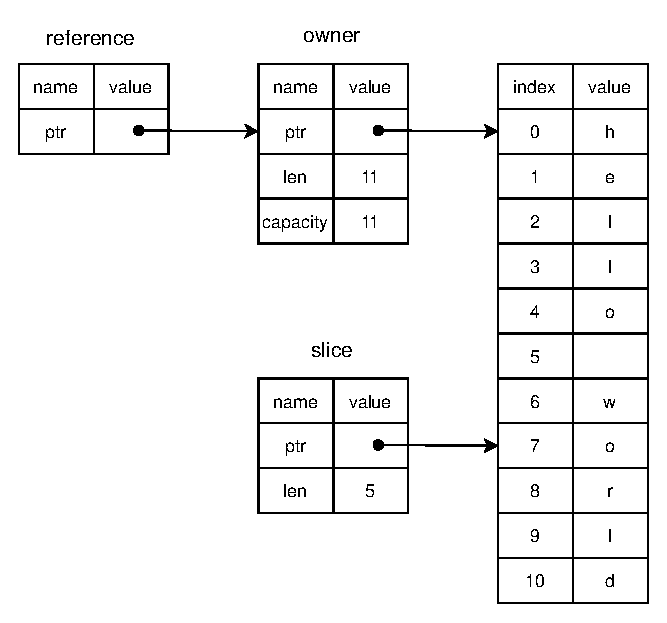
\includegraphics[width=0.5\textwidth]{images/own_ref_slice.eps}
                    \captionsetup{labelformat=empty}
                    % \caption{\textbf{}}
            \end{center}
        \end{figure}
    \end{minipage}      
    
    Each one may have \textcolor{blue}{different memory access time.}
\end{frame}

%%%%%%%%%%%%%%%%%%%%%%%%%%%%%%%%%%%%%%%%%%%%
%%%%%%%%%%%%%%%%%%%%%%%%%%%%%%%%%%%%%%%%%%%%
\begin{frame}[t, fragile]{Ownership}
    \vspace{-0.5cm}
    \begin{minipage}{0.7\linewidth}
    \begin{lstlisting}[language=Rust]
    let s = "app".to_string();
    let t = s;
    let u = s;
    \end{lstlisting}
    \end{minipage}     
    
        \begin{minipage}{0.3\linewidth}
            \begin{figure}[hp]
                \centering
                \begin{center}
                        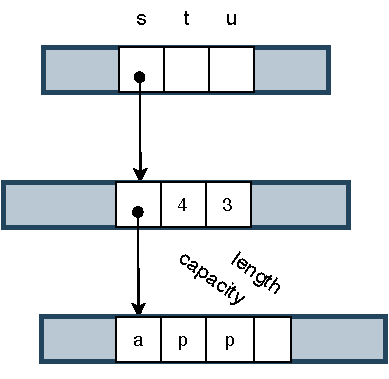
\includegraphics[width=1.0\textwidth]{images/owner1.pdf}
                        \captionsetup{labelformat=empty}
                        % \caption{\textbf{}}
                \end{center}
                
            \end{figure}
        \end{minipage}     
        \begin{minipage}{0.3\linewidth}
            \begin{figure}[hp]
                \centering
                \begin{center}
                        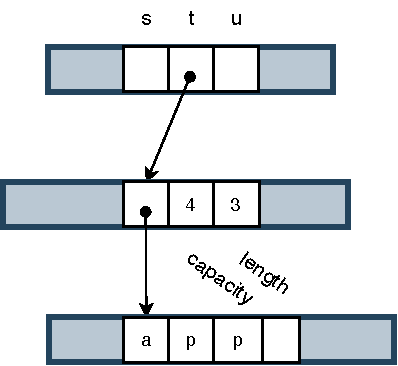
\includegraphics[width=1.0\textwidth]{images/owner2.pdf}
                        \captionsetup{labelformat=empty}
                        % \caption{\textbf{}}
                \end{center}
                
            \end{figure}
        \end{minipage}
        % \begin{minipage}{0.3\linewidth}
        %     \begin{figure}[hp]
        %         \centering
        %         \begin{center}
        %                 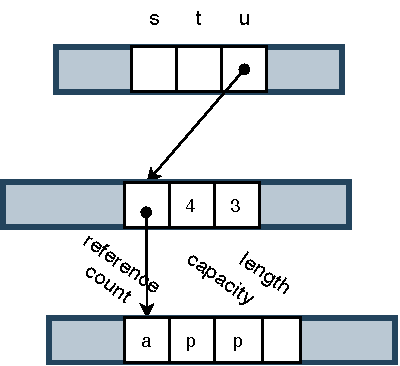
\includegraphics[width=1.0\textwidth]{images/owner3.pdf}
        %                 \captionsetup{labelformat=empty}
        %                 % \caption{\textbf{}}
        %         \end{center}
                
        %     \end{figure}
        % \end{minipage}

        \vspace{0.5cm}
        \begin{itemize}
            \item Each value is owned by single owner variable in Rust.
            \item Compiler error: \brownb{value "s" is dropped already.}
        \end{itemize}

 \end{frame}

%%%%%%%%%%%%%%%%%%%%%%%%%%%%%%%%%%%%%%%%%%%%
%%%%%%%%%%%%%%%%%%%%%%%%%%%%%%%%%%%%%%%%%%%%

\begin{frame}[t, fragile]{Advantage of Reference Counting}
\vspace{-0.5cm}
\begin{minipage}{0.7\linewidth}
\begin{lstlisting}[language=Rust]
let s = Rc::new("app".to_string());
let t = Rc::clone(&s);
let u = Rc::clone(&s); 
\end{lstlisting}
\end{minipage}     

    \begin{minipage}{0.3\linewidth}
        \begin{figure}[hp]
            \centering
            \begin{center}
                    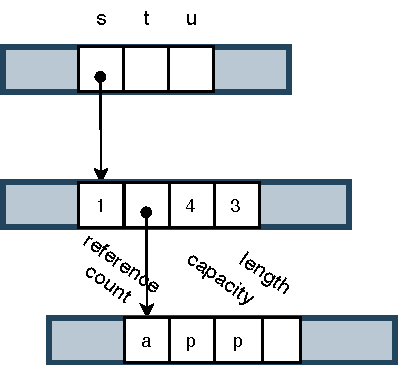
\includegraphics[width=1.0\textwidth]{images/rc1.pdf}
                    \captionsetup{labelformat=empty}
                    % \caption{\textbf{}}
            \end{center}
            
        \end{figure}
    \end{minipage}     
    \begin{minipage}{0.3\linewidth}
        \begin{figure}[hp]
            \centering
            \begin{center}
                    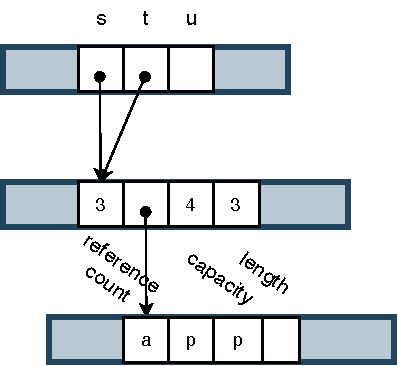
\includegraphics[width=1.0\textwidth]{images/rc2.pdf}
                    \captionsetup{labelformat=empty}
                    % \caption{\textbf{}}
            \end{center}
            
        \end{figure}
    \end{minipage}
    \begin{minipage}{0.3\linewidth}
        \begin{figure}[hp]
            \centering
            \begin{center}
                    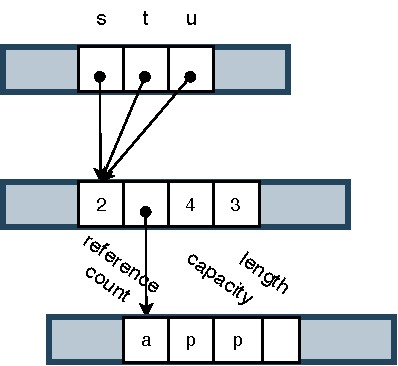
\includegraphics[width=1.0\textwidth]{images/rc3.pdf}
                    \captionsetup{labelformat=empty}
                    % \caption{\textbf{}}
            \end{center}
            
        \end{figure}
    \end{minipage}
    \vspace{0.5cm}

    \textbf{Advantage}
    \begin{itemize}
        \item \blue{Sharing ownership} 
        \begin{itemize}
            \item Each value is owned by single owner variable in Rust.
        \end{itemize}
        \item \blue{Dynamic memory de/allocation}
        \begin{itemize}
            \item Rust usually determine lifetime of variable at compile time. 
        \end{itemize}
    \end{itemize}
\end{frame}

%%%%%%%%%%%%%%%%%%%%%%%%%%%%%%%%%%%%%%%%%%%%
%%%%%%%%%%%%%%%%%%%%%%%%%%%%%%%%%%%%%%%%%%%%

\begin{frame}[fragile]{Disadvantge of Reference Counting}
    
\vspace{-0.5cm}
\begin{minipage}{0.7\linewidth}
\begin{lstlisting}[language=Rust]
let s = Rc::new("app".to_string());
let t = Rc::clone(&s);
let u = Rc::clone(&s); 
\end{lstlisting}
\end{minipage}      

    \begin{minipage}{0.3\linewidth}
        \begin{figure}[hp]
            \centering
            \begin{center}
                    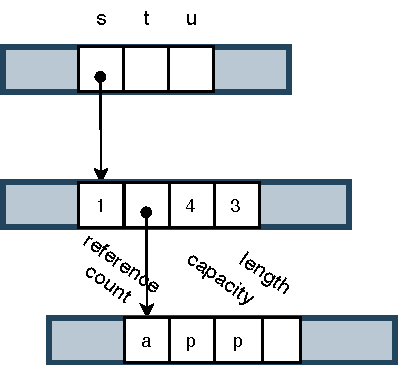
\includegraphics[width=1.0\textwidth]{images/rc1.pdf}
                    \captionsetup{labelformat=empty}
                    % \caption{\textbf{}}
            \end{center}
            
        \end{figure}
    \end{minipage}     
    \begin{minipage}{0.3\linewidth}
        \begin{figure}[hp]
            \centering
            \begin{center}
                    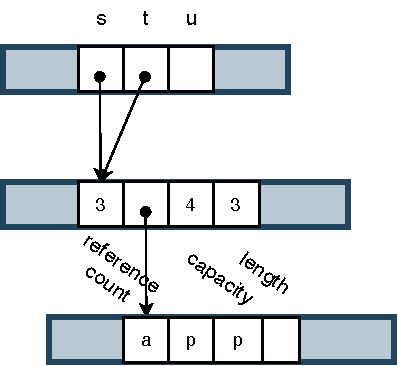
\includegraphics[width=1.0\textwidth]{images/rc2.pdf}
                    \captionsetup{labelformat=empty}
                    % \caption{\textbf{}}
            \end{center}
            
        \end{figure}
    \end{minipage}
    \begin{minipage}{0.3\linewidth}
        \begin{figure}[hp]
            \centering
            \begin{center}
                    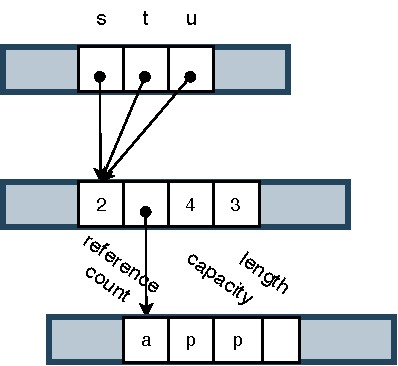
\includegraphics[width=1.0\textwidth]{images/rc3.pdf}
                    \captionsetup{labelformat=empty}
                    % \caption{\textbf{}}
            \end{center}
            
        \end{figure}
    \end{minipage}
    \vspace{0.5cm}

    \textbf{Disadvantage}
    \begin{itemize}
        \item \blue{Need to check reference count} 
        \item \blue{Heap allocation}
    \end{itemize}


\end{frame}


%%%%%%%%%%%%%%%%%%%%%%%%%%%%%%%%%%%%%%%%%%%%
%%%%%%%%%%%%%%%%%%%%%%%%%%%%%%%%%%%%%%%%%%%%

\begin{frame}[fragile]{Problem Description}
    
    In this thesis, our goal is to determine the magnitude of performance change regarding the following aspects on overall performance of Big Data processing.
     
    \vspace{0.5cm}
    \begin{itemize}
        
        \item \blue{High Complex Nested Objects vs. Simple Objects/Primitive Types using  different memory strategies: Ownership vs. Borrowing vs. Slicing vs. Reference Counting}
        \item \blue{Automated Reference Counting (Rc) vs. Normal Reference}
        \item \blue{Multithreading using Atomic Reference Counting (Arc) vs. Normal Reference}
        \item \blue{Arc vs. Deep Copy}
    \end{itemize}
    
    We have specified 5 different experiments. 
    
\end{frame}




%%%%%%%%%%%%%%%%%%%%%%%%%%%%%%%%%%%%%%%%%%%%
%%%%%%%%%%%%%%%%%%%%%%%%%%%%%%%%%%%%%%%%%%%%


\begin{frame}[fragile]{Complex Object - Memory Ownership and Borrowing}

A Complex Object like a nested Customer Object like those defined in the complete Web-based shop. 
 
\begin{minipage}{0.5\linewidth}
\centering
\begin{lstlisting}[language=Rust]
struct CustomerOwned {
    key: i32,
    total_purchase: f64,
    zip_code: String,
    order: OrderOwned,
    ... 10 more
    }
\end{lstlisting}
\end{minipage}\hfill  
\begin{minipage}{0.5\linewidth}
\centering
\begin{itemize}
    \item \blue{All fields are owners.} 
\end{itemize}
\end{minipage}

\begin{minipage}{0.5\linewidth}
\centering
\begin{lstlisting}[language=Rust]
struct CustomerBorrowed<'a> {
    key: &'a i32,
    total_purchase: &'a f64,
    zip_code: &'a String,
    order: &'a OrderBorrowed<'a>,
    ... 10 more 
    }
\end{lstlisting}
\end{minipage}\hfill  
\begin{minipage}{0.5\linewidth}
\centering
\begin{itemize}
    \item \blue{All fields are references.}
    \item \blue{'a} is lifetime specifier.
    \item Rust compiler cannot determine \blue{lifetime} automatically.
\end{itemize}
\end{minipage}
\end{frame}
%%%%%%%%%%%%%%%%%%%%%%%%%%%%%%%%%%%%%%%%%%%%
%%%%%%%%%%%%%%%%%%%%%%%%%%%%%%%%%%%%%%%%%%%%

\begin{frame}[t,fragile]{Complex Object - Slicing and Reference Counting}

%Memory Slicing and Atomic Reference Counting 
\begin{minipage}{0.5\linewidth}
\centering
\begin{lstlisting}[language=Rust]
struct CustomerSlice<'a> {
    key: &'a i32,
    total_purchase: &'a f64,
    zip_code: &'a str,
    order: &'a OrderSlice<'a>
    ... 10 more 
    }
\end{lstlisting}
\end{minipage}\hfill  
\begin{minipage}{0.5\linewidth}
\centering
\begin{itemize}
    \item \blue{Fields are mix of references and slices.} 
    \item Slice is obtained only for \blue{contiguously allocated data structure}, such as String and Vec.
\end{itemize}
\end{minipage}

\begin{minipage}{0.5\linewidth}
\centering
\begin{lstlisting}[language=Rust]
struct CustomerRc {
    key: Rc<i32>,
    total_purchase: Rc<f64>,
    zip_code: Rc<String>,
    order: Rc<OrderRc>
    ... 10 more 
    }
\end{lstlisting}
\end{minipage}\hfill  
\begin{minipage}{0.5\linewidth}
\centering
\begin{itemize}
    \item \blue{All fields are Reference Counting}
\end{itemize}
\end{minipage}
    
\end{frame}

%%%%%%%%%%%%%%%%%%%%%%%%%%%%%%%%%%%%%%%%%%%%
%%%%%%%%%%%%%%%%%%%%%%%%%%%%%%%%%%%%%%%%%%%%

\begin{frame}[fragile]{Multithreading with Atomic Reference Counting}
    Atomic Reference Counting

    \vspace{0.5cm}
    \textbf{Advantage}
    \begin{itemize}
        \item \blue{Sharing ownership} 
        \item \blue{Dynamic memory de/allocation}
        \item \blue{Sharing among multithreads}
    \end{itemize}

    \vspace{0.5cm}

    \textbf{Disadvantage}
    \begin{itemize}
        \item \blue{Need to check reference count} 
        \item \blue{Heap allocation}
        \item \blue{Atomic operation} 
    \end{itemize}

\end{frame}

%%%%%%%%%%%%%%%%%%%%%%%%%%%%%%%%%%%%%%%%%%%%
%%%%%%%%%%%%%%%%%%%%%%%%%%%%%%%%%%%%%%%%%%%%

\begin{frame}[fragile]{Impact of Memory Management on performance of Big Data Processing}

    
\blueb{Merge-sort}
\begin{itemize}
    \item Many contiguous memory de/allocations
    \item Common memory usage pattern in sorting algorithms for Big Data Processing.
    \begin{itemize}
        \item  ex. External-sort
    \end{itemize}
\end{itemize}

\end{frame}

%%%%%%%%%%%%%%%%%%%%%%%%%%%%%%%%%%%%%%%%%%%%
%%%%%%%%%%%%%%%%%%%%%%%%%%%%%%%%%%%%%%%%%%%%

\begin{frame}[fragile]{Impact of Memory Management on performance of Big Data Processing}
\blueb{Tree-aggtegate}
\begin{itemize}
    \item Many intermediate HashMap like data structures
    \item Many de/allocations of intermediate data
    \item Common memory and network usage pattern in Big Data Processing
\end{itemize}

\begin{figure}[htb]
    \begin{minipage}[t]{0.5\linewidth}\centering
        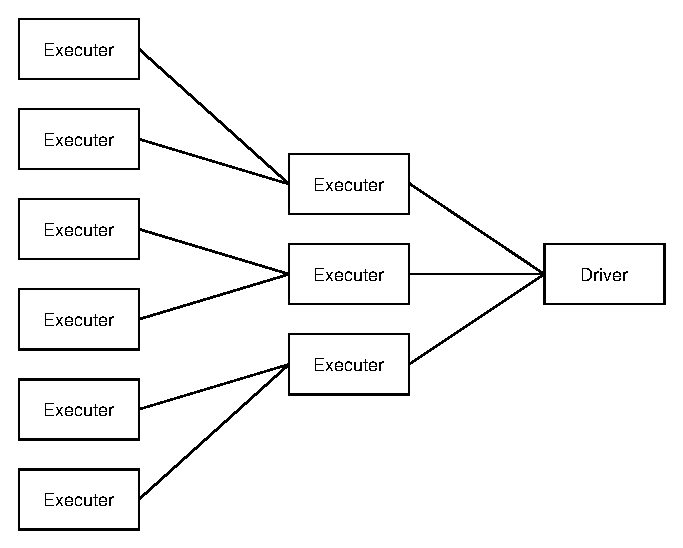
\includegraphics[width=7cm]{images/tree_agg.eps} 
    \end{minipage}
\end{figure}

\end{frame}

%%%%%%%%%%%%%%%%%%%%%%%%%%%%%%%%%%%%%%%%%%%%
%%%%%%%%%%%%%%%%%%%%%%%%%%%%%%%%%%%%%%%%%%%%
\begin{frame}[fragile]{Impact of Memory Management on performance of Big Data Processing}
    \blueb{K-Nearest-Neighbors (KNN)}
    \begin{itemize}
        \item An example of Machine Learning algorithm that requires Big Data processing.
        \item Text document classification 
        \item We are interested only in preprocessing phase.
        \item String manipulations
        \item It is just matrix read operation after preprocessing phase.
    \end{itemize}    

\end{frame}

%%%%%%%%%%%%%%%%%%%%%%%%%%%%%%%%%%%%%%%%%%%%
%%%%%%%%%%%%%%%%%%%%%%%%%%%%%%%%%%%%%%%%%%%%

% 
% \begin{frame}[fragile]{Problem Description}
%     Our goal is to determine the magnitude of performance change regarding the following aspects. 
%     \vspace{0.5cm}
%     \begin{itemize}
%         \item \blue{Memory Management for High Complex Nested Objects}
%         \item \blue{Different Rust Memory Management Strategies}
%         \item \blue{Automated Reference Counting (Rc) vs. Reference}
%         \item \blue{Multithreading using Atomic Reference Counting (Arc)}
%         \item \blue{Arc vs. Deep Copy on Overall Performance of Big Data Processing}
%     \end{itemize}
% \end{frame}

%%%%%%%%%%%%%%%%%%%%%%%%%%%%%%%%%%%%%%%%%%%%
%%%%%%%%%%%%%%%%%%%%%%%%%%%%%%%%%%%%%%%%%%%%

\begin{frame}[t, fragile]{Experimental Setting}
    
    \textbf{Machine Specification}
    \begin{itemize}
        \item Google Cloud Platform: n1-standard-8
        \item CPU : 8 cores
        \item RAM: 30 GB
        \item Standard persistent disk: 10 GB
    \end{itemize}
    \textbf{Data Set}
    \begin{itemize}
        \item Randomized generated data of \textbf{Customer objects} (Synthetic Data)
        \begin{itemize}
            \item CustomerOwned
            \item CustomerBorrowed
            \item CustomerSlice
            \item CustomerRc
        \end{itemize} 
        \item \textbf{Wikipedia Text data} set (Real-World Data)
        \begin{itemize}
            \item Training set: \(100 \times 10^3 \) wiki pages
            \item Testing set: \(18 \times  10^3\) wiki pages
        \end{itemize} 
    \end{itemize} 
    \textbf{Execution}
    \begin{itemize}
        \item Run each experiment 5 time 
        \item Take average of the 5 runs 
    \end{itemize}
\end{frame}

%%%%%%%%%%%%%%%%%%%%%%%%%%%%%%%%%%%%%%%%%%%%
%%%%%%%%%%%%%%%%%%%%%%%%%%%%%%%%%%%%%%%%%%%%

\begin{frame}[fragile]{Experiment 1: Accessing Object with Different Variable Type}

    \textbf{Question}
    \begin{itemize}
        % \item How much does selection of different memory management strategies differ memory access time?
        \item What is the proformance differences among different memory management strategies?
    \end{itemize}

    \vspace{0.5cm}

    \textbf{Evaluation}
    \begin{itemize}
        \item \blueb{Construct Complex objects}
        \item With different memory management strategies like \blueb{Owner, Reference, Slice}
        \item \textbf{CustomerOwned} vs. \textbf{CustomerBorrowed} vs. \textbf{CustomerSlice}
        \item Measure access time of different \blueb{fields of complex objects}
    \end{itemize}

\end{frame}

%%%%%%%%%%%%%%%%%%%%%%%%%%%%%%%%%%%%%%%%%%%%
%%%%%%%%%%%%%%%%%%%%%%%%%%%%%%%%%%%%%%%%%%%%
% 
% \begin{frame}[t, fragile]{Experiment 1: Accessing Object with Different Variable Type}
%     \vspace{-0.7cm}
%     \begin{figure}[hp]
%         \centering
%         \begin{center}
%                 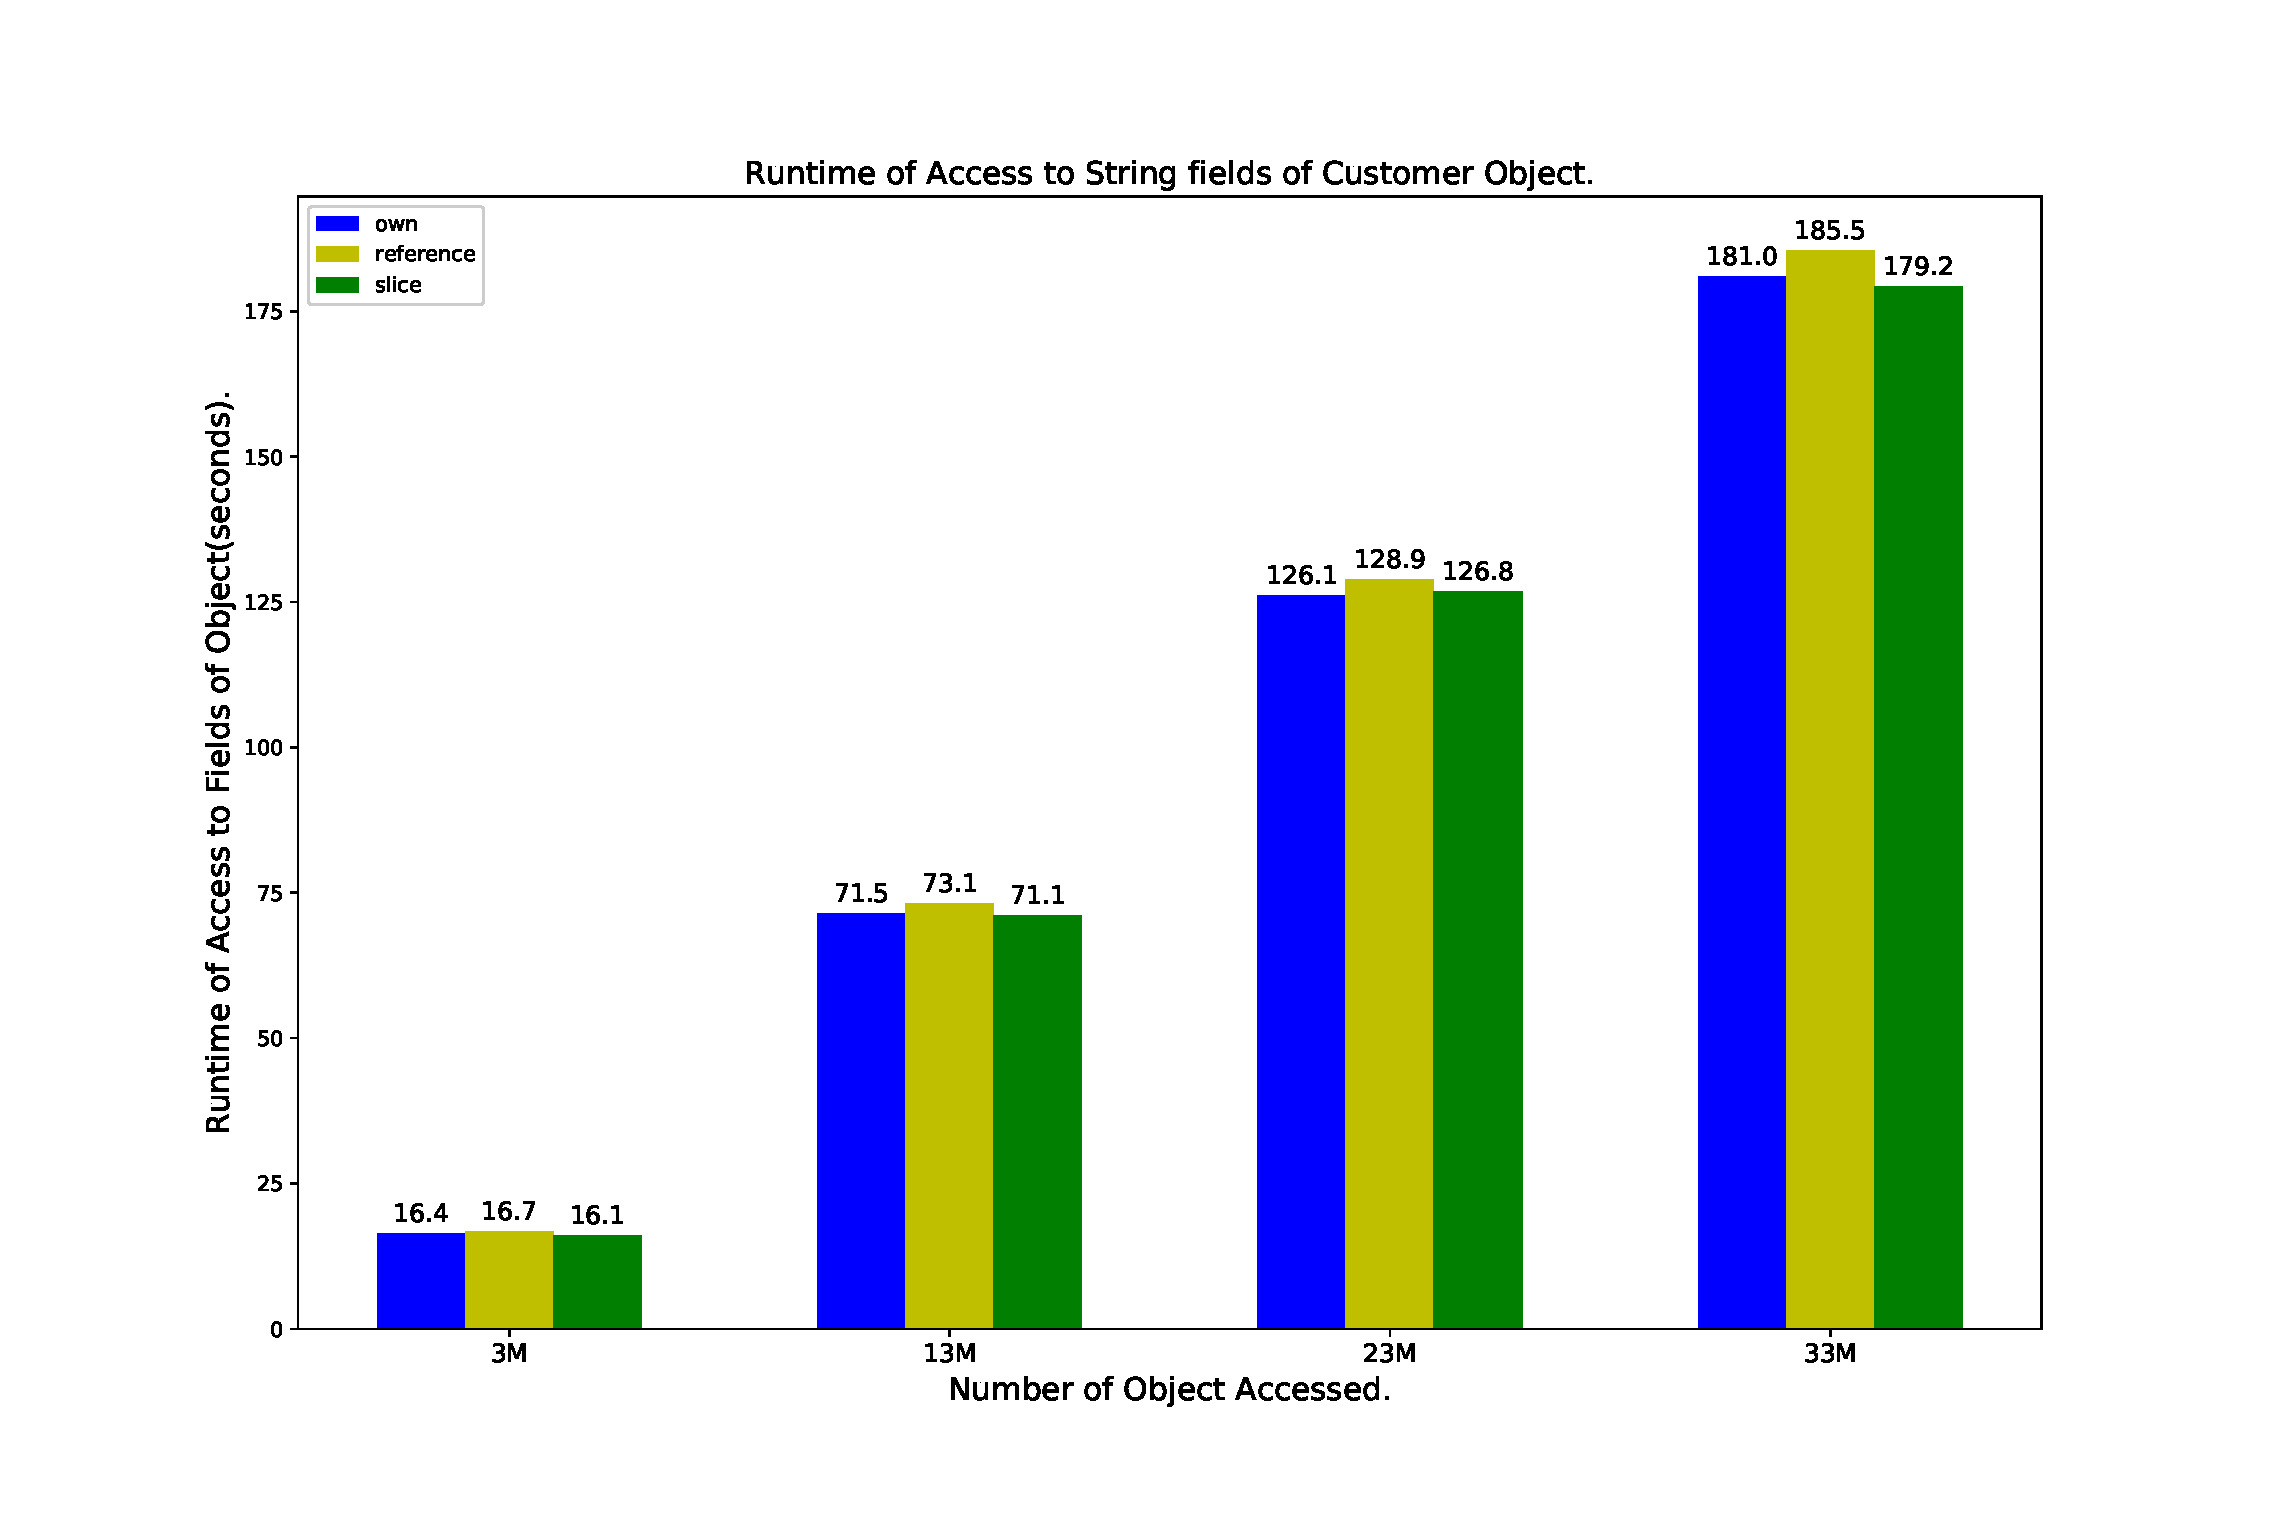
\includegraphics[width=1\textwidth]{images/rust_access_different_poniter_init.eps}
%                 \captionsetup{labelformat=empty}
%                 % \caption{\textbf{}}
%         \end{center}
%     \end{figure}
% 
% \end{frame}

%%%%%%%%%%%%%%%%%%%%%%%%%%%%%%%%%%%%%%%%%%%%
%%%%%%%%%%%%%%%%%%%%%%%%%%%%%%%%%%%%%%%%%%%%

\begin{frame}[t, fragile]{Experiment 1: Accessing Object with Different Variable Type}
    \vspace{-0.7cm}
    \begin{figure}[hp]
        \centering
        \begin{center}
                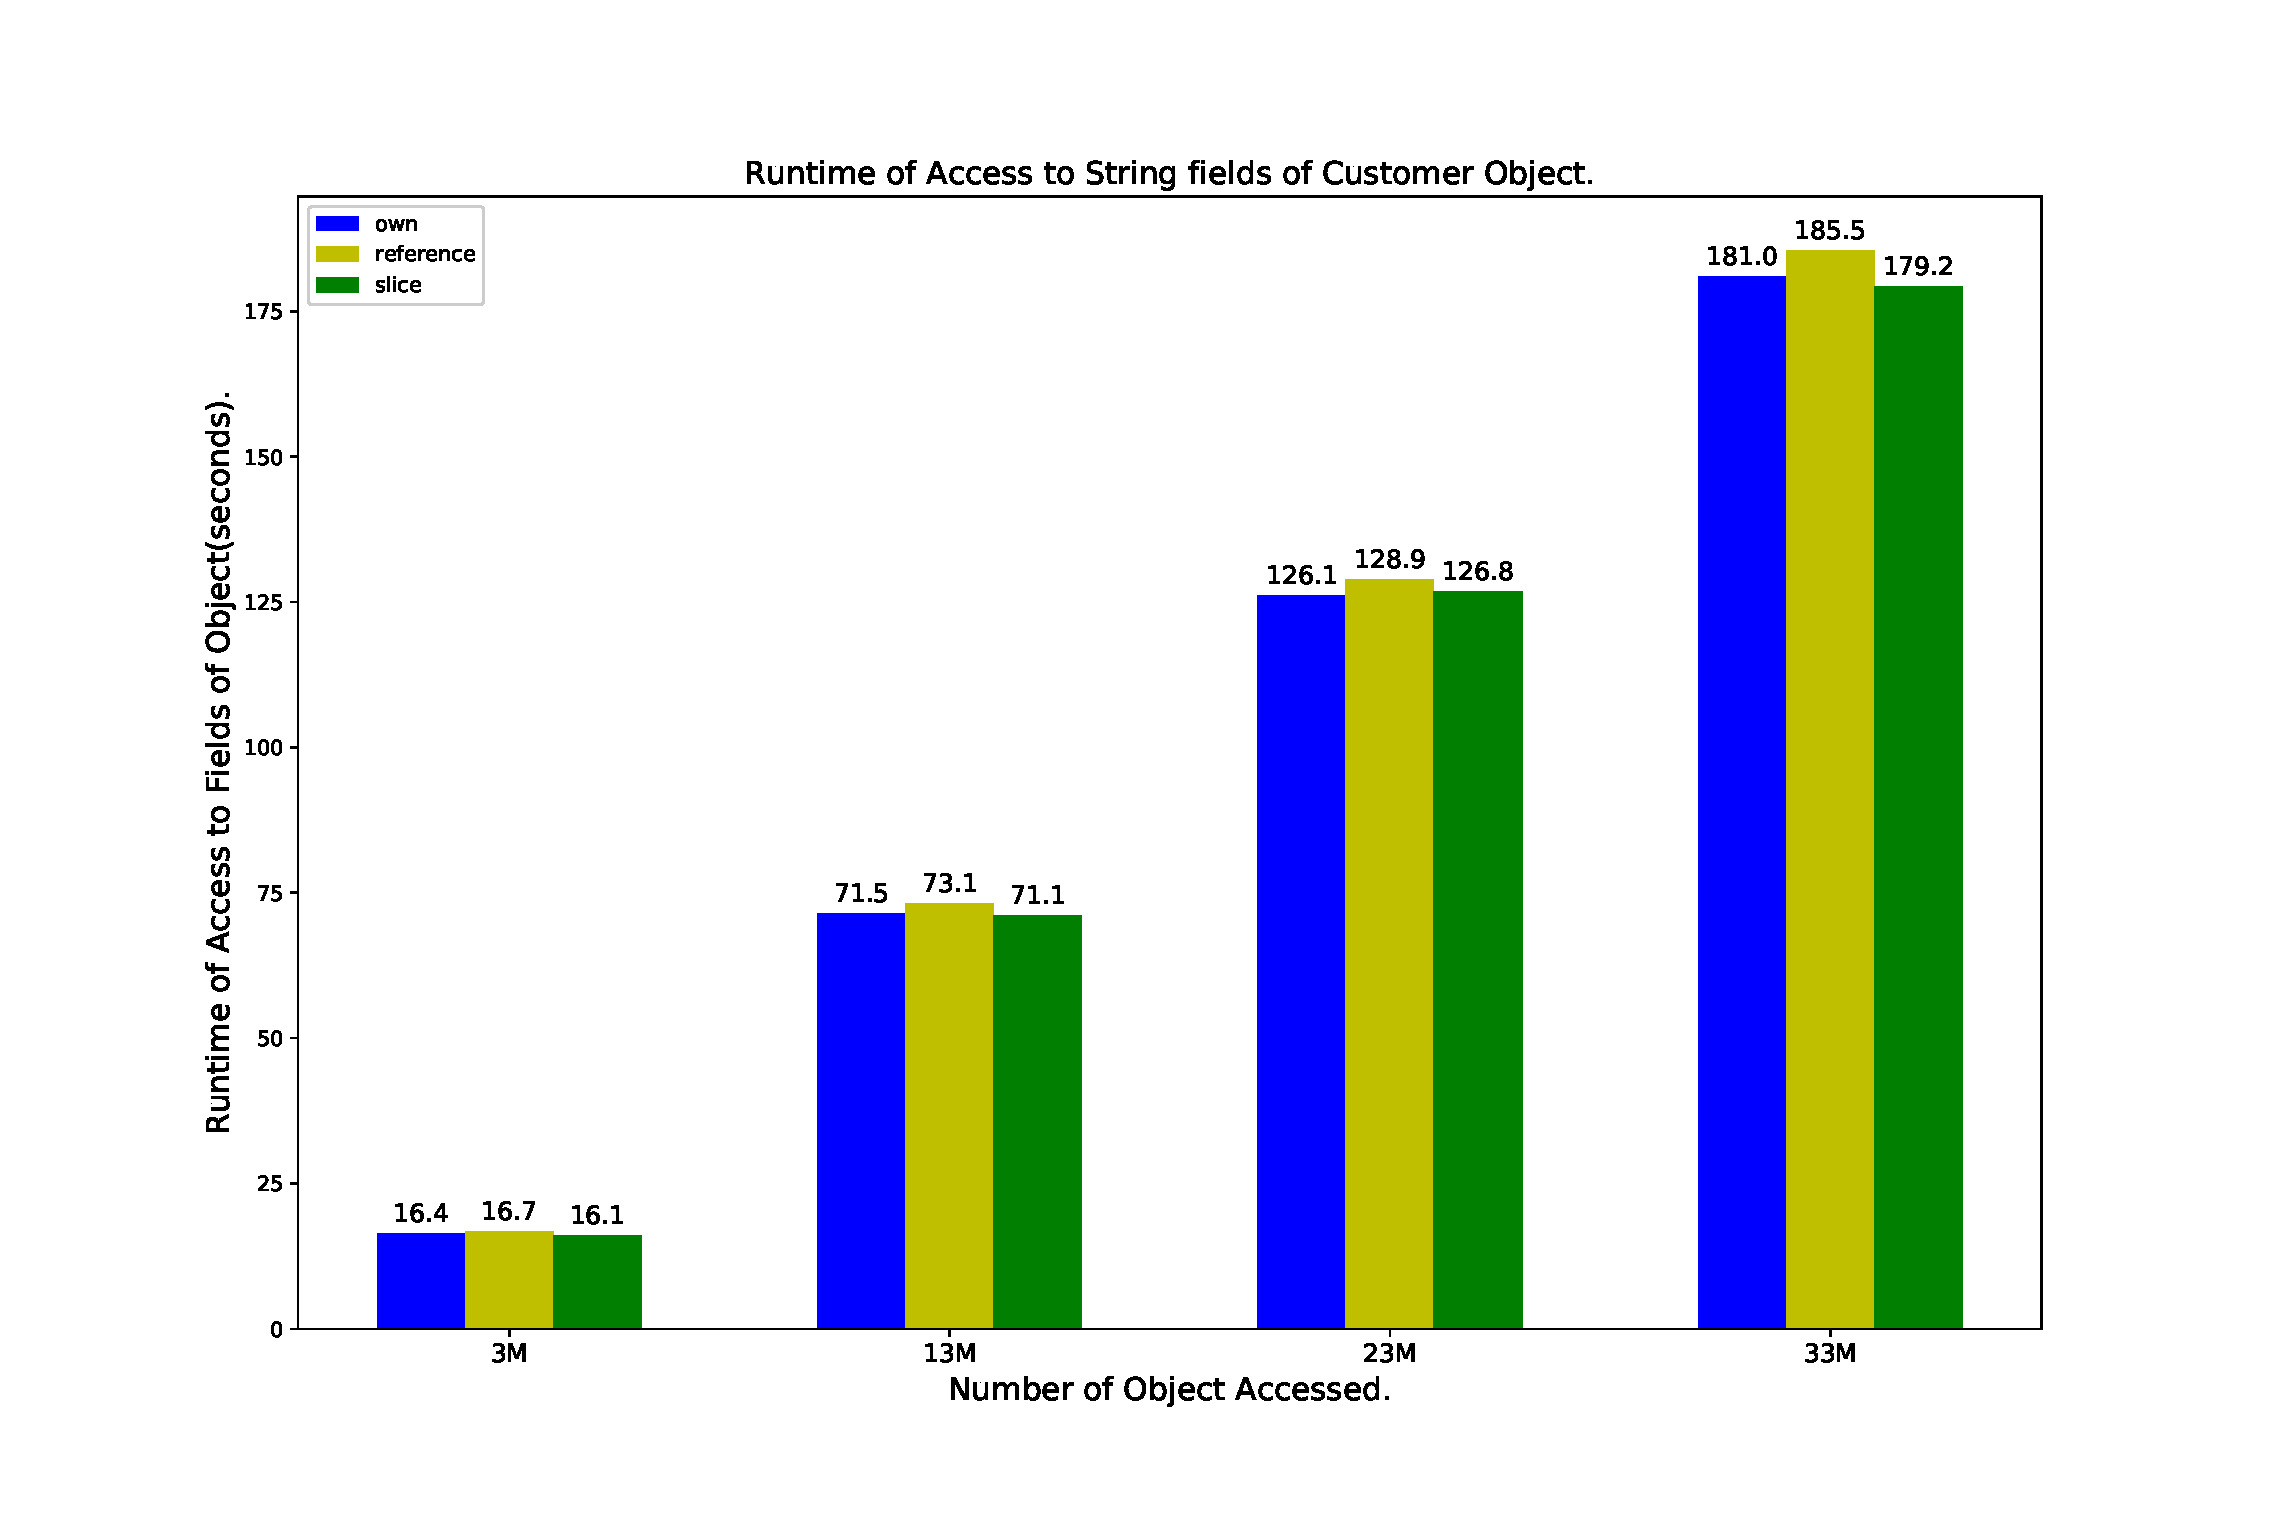
\includegraphics[width=0.8\textwidth]{images/rust_access_different_poniter_init.eps}
                \captionsetup{labelformat=empty}
                % \caption{\textbf{}}
        \end{center}
    \end{figure}
    \vspace{-1cm}
    \textbf{Result}
    \begin{itemize}
        \item No differences of memory access time among Customer objects using different memory management strategies.
    \end{itemize}
    \textbf{Discussion}
    \begin{itemize}
        \item Selection of different memory management strategies does not have impact on memory access time.
    \end{itemize}

\end{frame}

%%%%%%%%%%%%%%%%%%%%%%%%%%%%%%%%%%%%%%%%%%%%
%%%%%%%%%%%%%%%%%%%%%%%%%%%%%%%%%%%%%%%%%%%%

\begin{frame}[fragile]{Experiment 2: Assessment of different reference methods in Rust}

    \textbf{Question}
    \begin{itemize}
        \item How much does Reference Counting hits performance?
    \end{itemize}

    \vspace{0.5cm}

    \textbf{Evaluation}
    \begin{itemize}
        \item \blueb{Construct complex objects}
        \item \blueb{Reference Counting} vs \blueb{reference}
        \item CustomerRc vs. CustomerBorrowed
        \item Measure time to \blueb{drop variables of complex objects}
    \end{itemize}

\end{frame}

%%%%%%%%%%%%%%%%%%%%%%%%%%%%%%%%%%%%%%%%%%%%
%%%%%%%%%%%%%%%%%%%%%%%%%%%%%%%%%%%%%%%%%%%%

% 
% \begin{frame}[fragile]{Experiment 2: Assessment of different reference methods in Rust}
%     \vspace{-0.5cm}
%     \begin{figure}[hp]
%         \centering
%         \begin{center}
%                 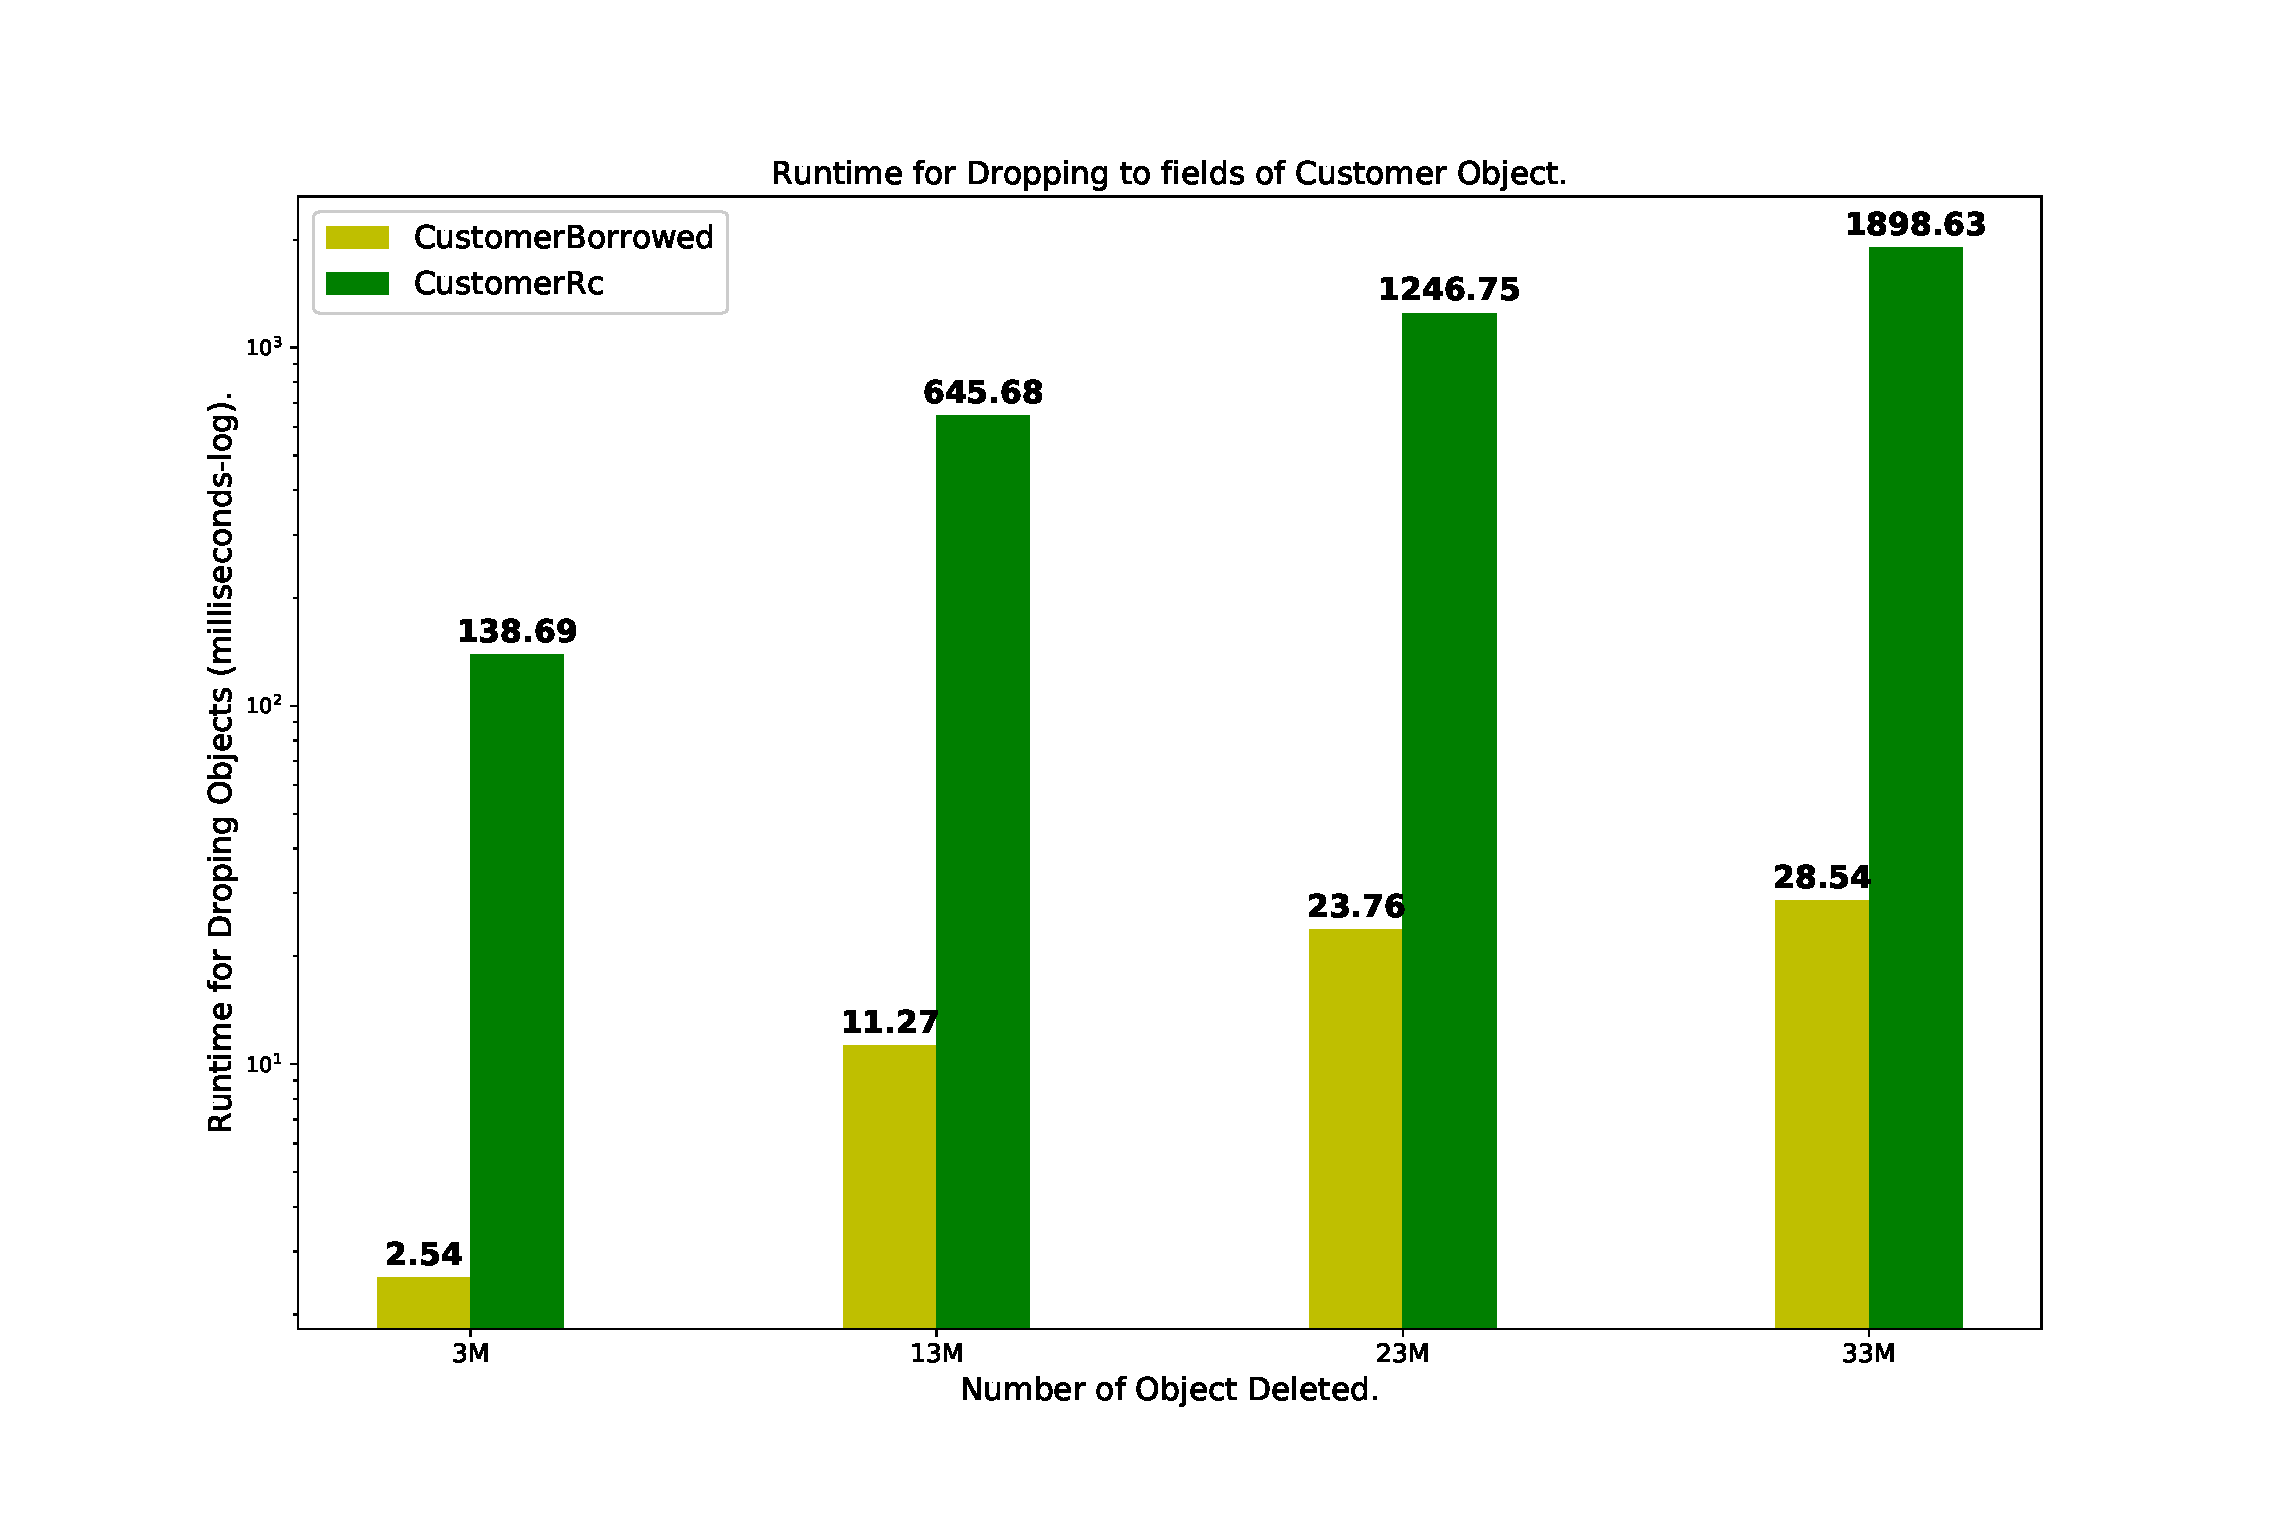
\includegraphics[width=1\textwidth]{images/rust_droptime_borring_rc.eps}
%                 \captionsetup{labelformat=empty}
%                 % \caption{\textbf{}}
%         \end{center}
%     \end{figure}
% \end{frame}
%%%%%%%%%%%%%%%%%%%%%%%%%%%%%%%%%%%%%%%%%%%%
%%%%%%%%%%%%%%%%%%%%%%%%%%%%%%%%%%%%%%%%%%%%

\begin{frame}[fragile]{Experiment 2: Assessment of different reference methods in Rust}
    \vspace{-0.5cm}
    \begin{figure}[hp]
        \centering
        \begin{center}
                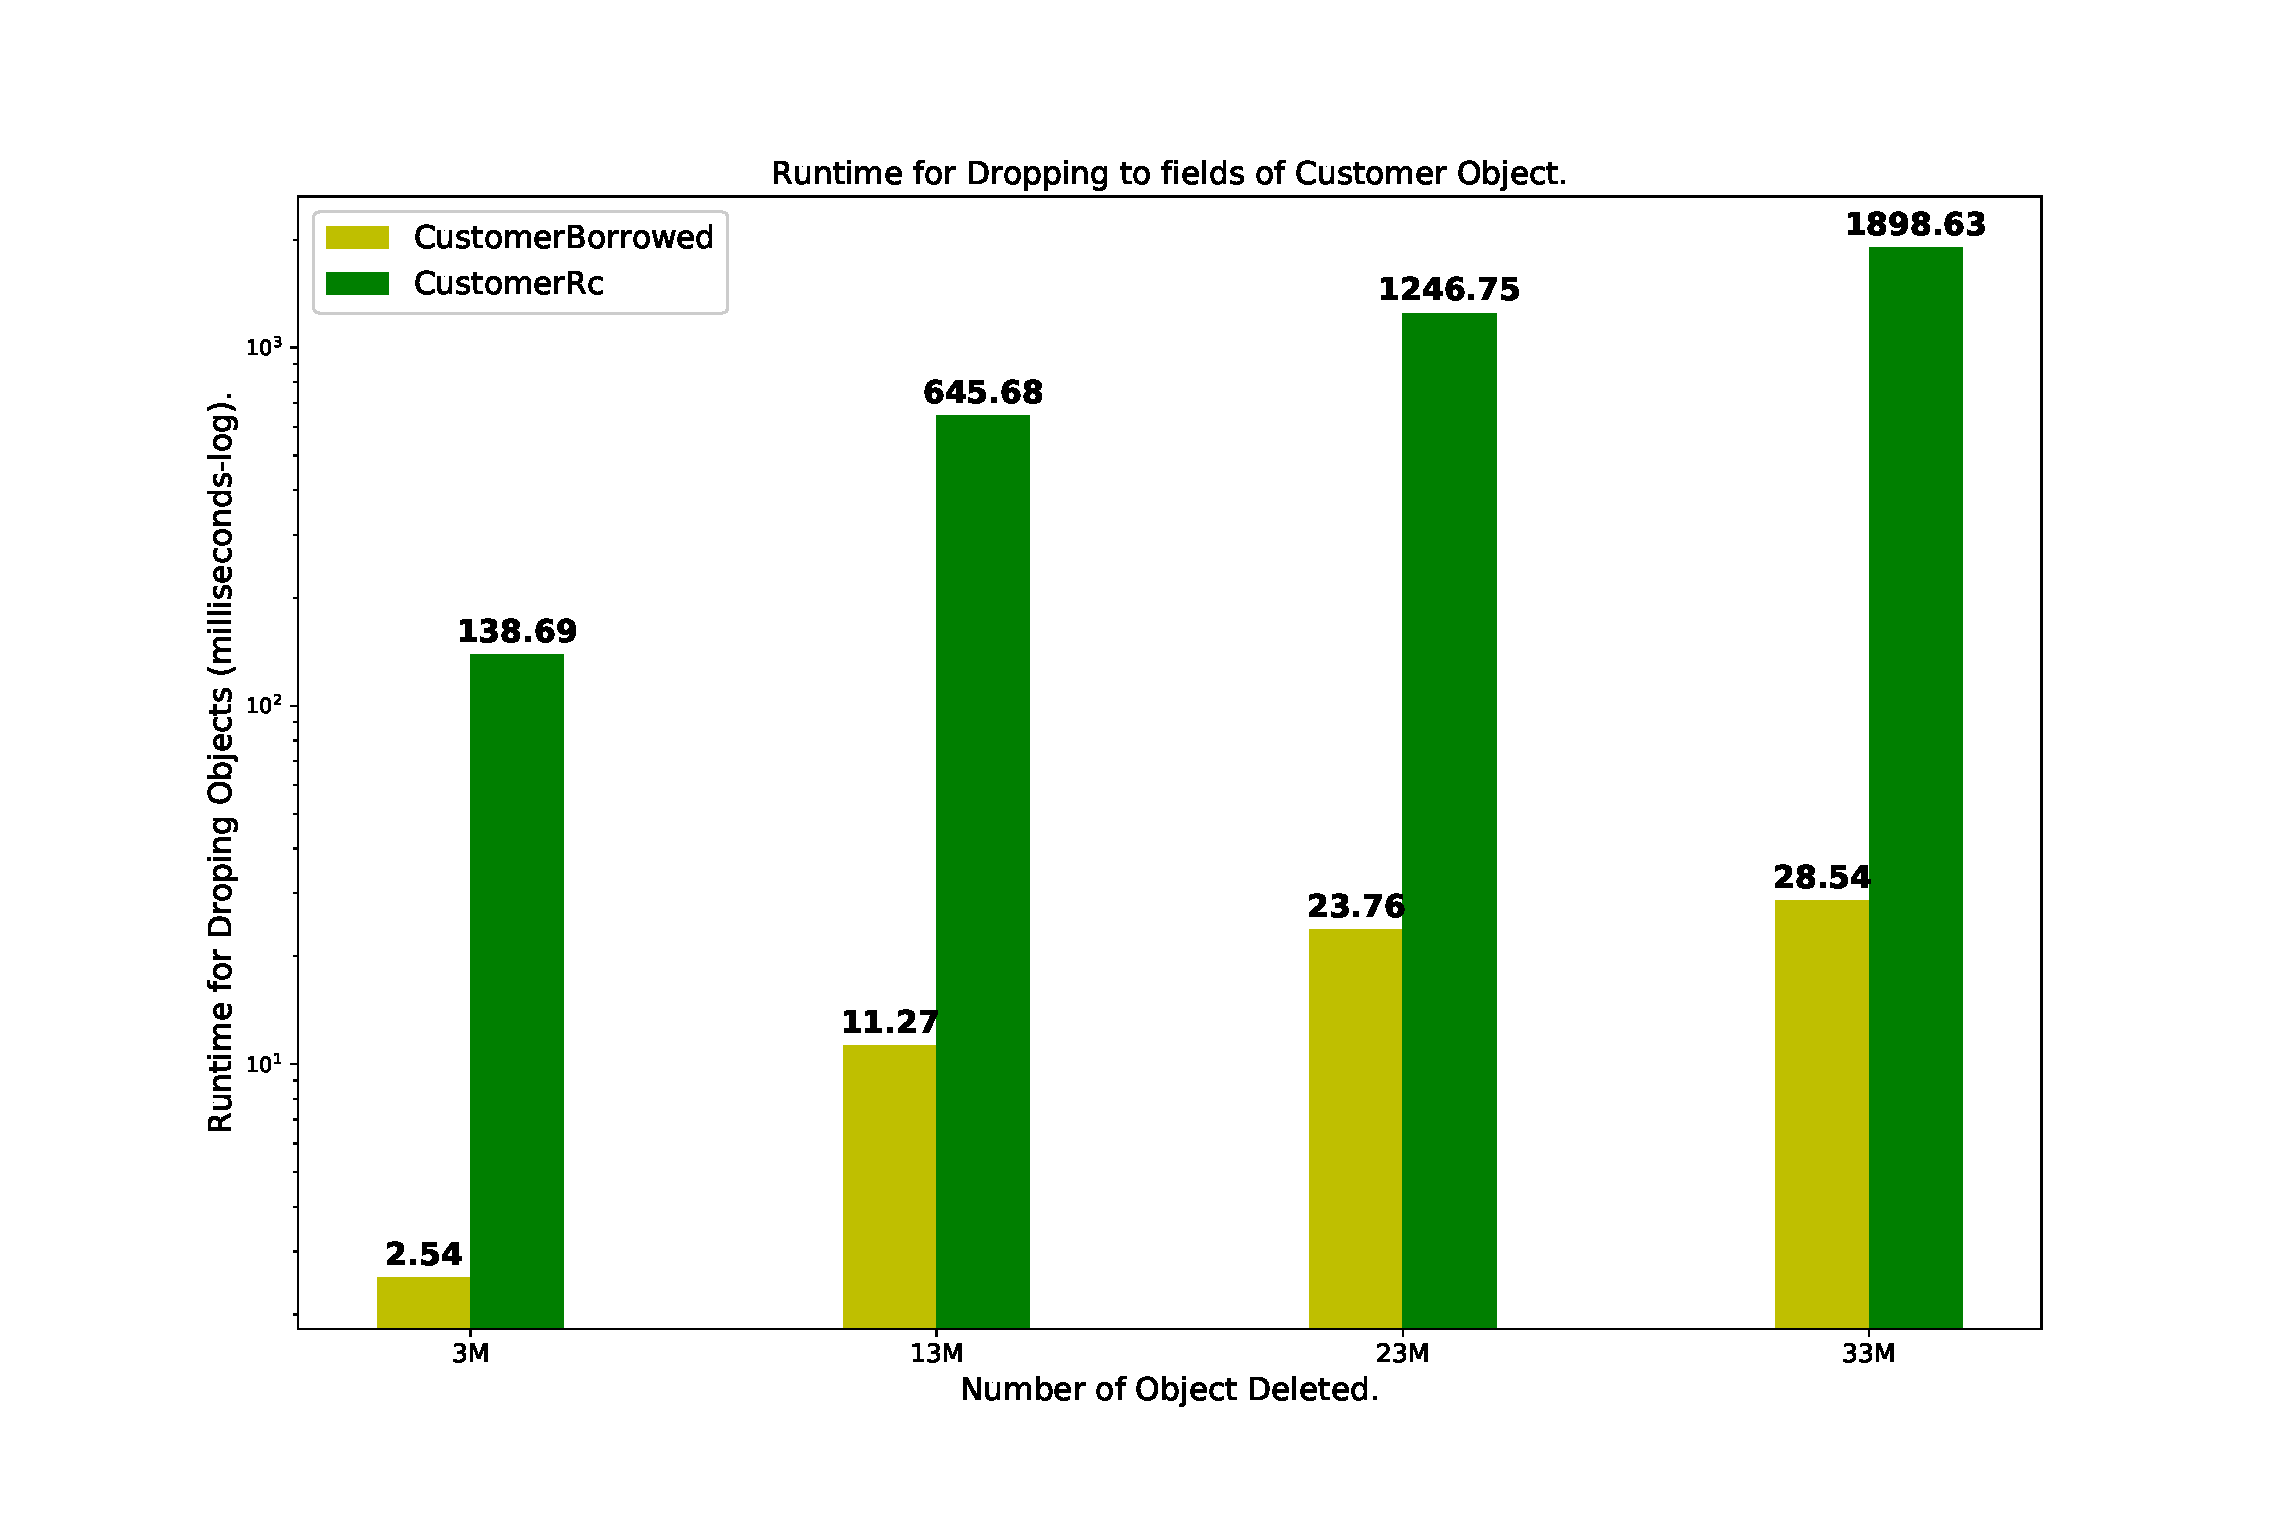
\includegraphics[width=0.8\textwidth]{images/rust_droptime_borring_rc.eps}
                \captionsetup{labelformat=empty}
                % \caption{\textbf{}}
        \end{center}
    \end{figure}
\vspace{-0.5cm}
    \textbf{Result}
    \begin{itemize}
        \item Dropping Reference Counting is about \blueb{60 times slower} than normal reference.
    \end{itemize}
    \textbf{Discussion}
    \begin{itemize}
        \item Reference Counting needs some CPU cycles to check reference count.
        \item In complex objects, overhead is significant.
    \end{itemize}
\end{frame}

%%%%%%%%%%%%%%%%%%%%%%%%%%%%%%%%%%%%%%%%%%%%
%%%%%%%%%%%%%%%%%%%%%%%%%%%%%%%%%%%%%%%%%%%%

\begin{frame}[fragile]{Experiment 3: Merge-Sort}

    \textbf{Question}
    \begin{itemize}
        \item What is performance hit of Merge-Sort algorithm using Arc vs, normal reference?
    \end{itemize}

    \vspace{0.5cm}

    \textbf{Evaluation}
    \begin{itemize}
        \item Share \blueb{vector} of complex objects in multithreads
        \item \blueb{Atomic Reference Counting (Arc)} vs. \blueb{normal reference}
        \item Measure \blueb{runtime of merge-sort algorithms}
    \end{itemize}
\end{frame}

%%%%%%%%%%%%%%%%%%%%%%%%%%%%%%%%%%%%%%%%%%%%
%%%%%%%%%%%%%%%%%%%%%%%%%%%%%%%%%%%%%%%%%%%%

% 
% \begin{frame}[fragile]{Experiment 3: Merge-sort}
%     \vspace{-0.7cm}
%     \begin{figure}[hp]
%         \centering
%         \begin{center}
%                 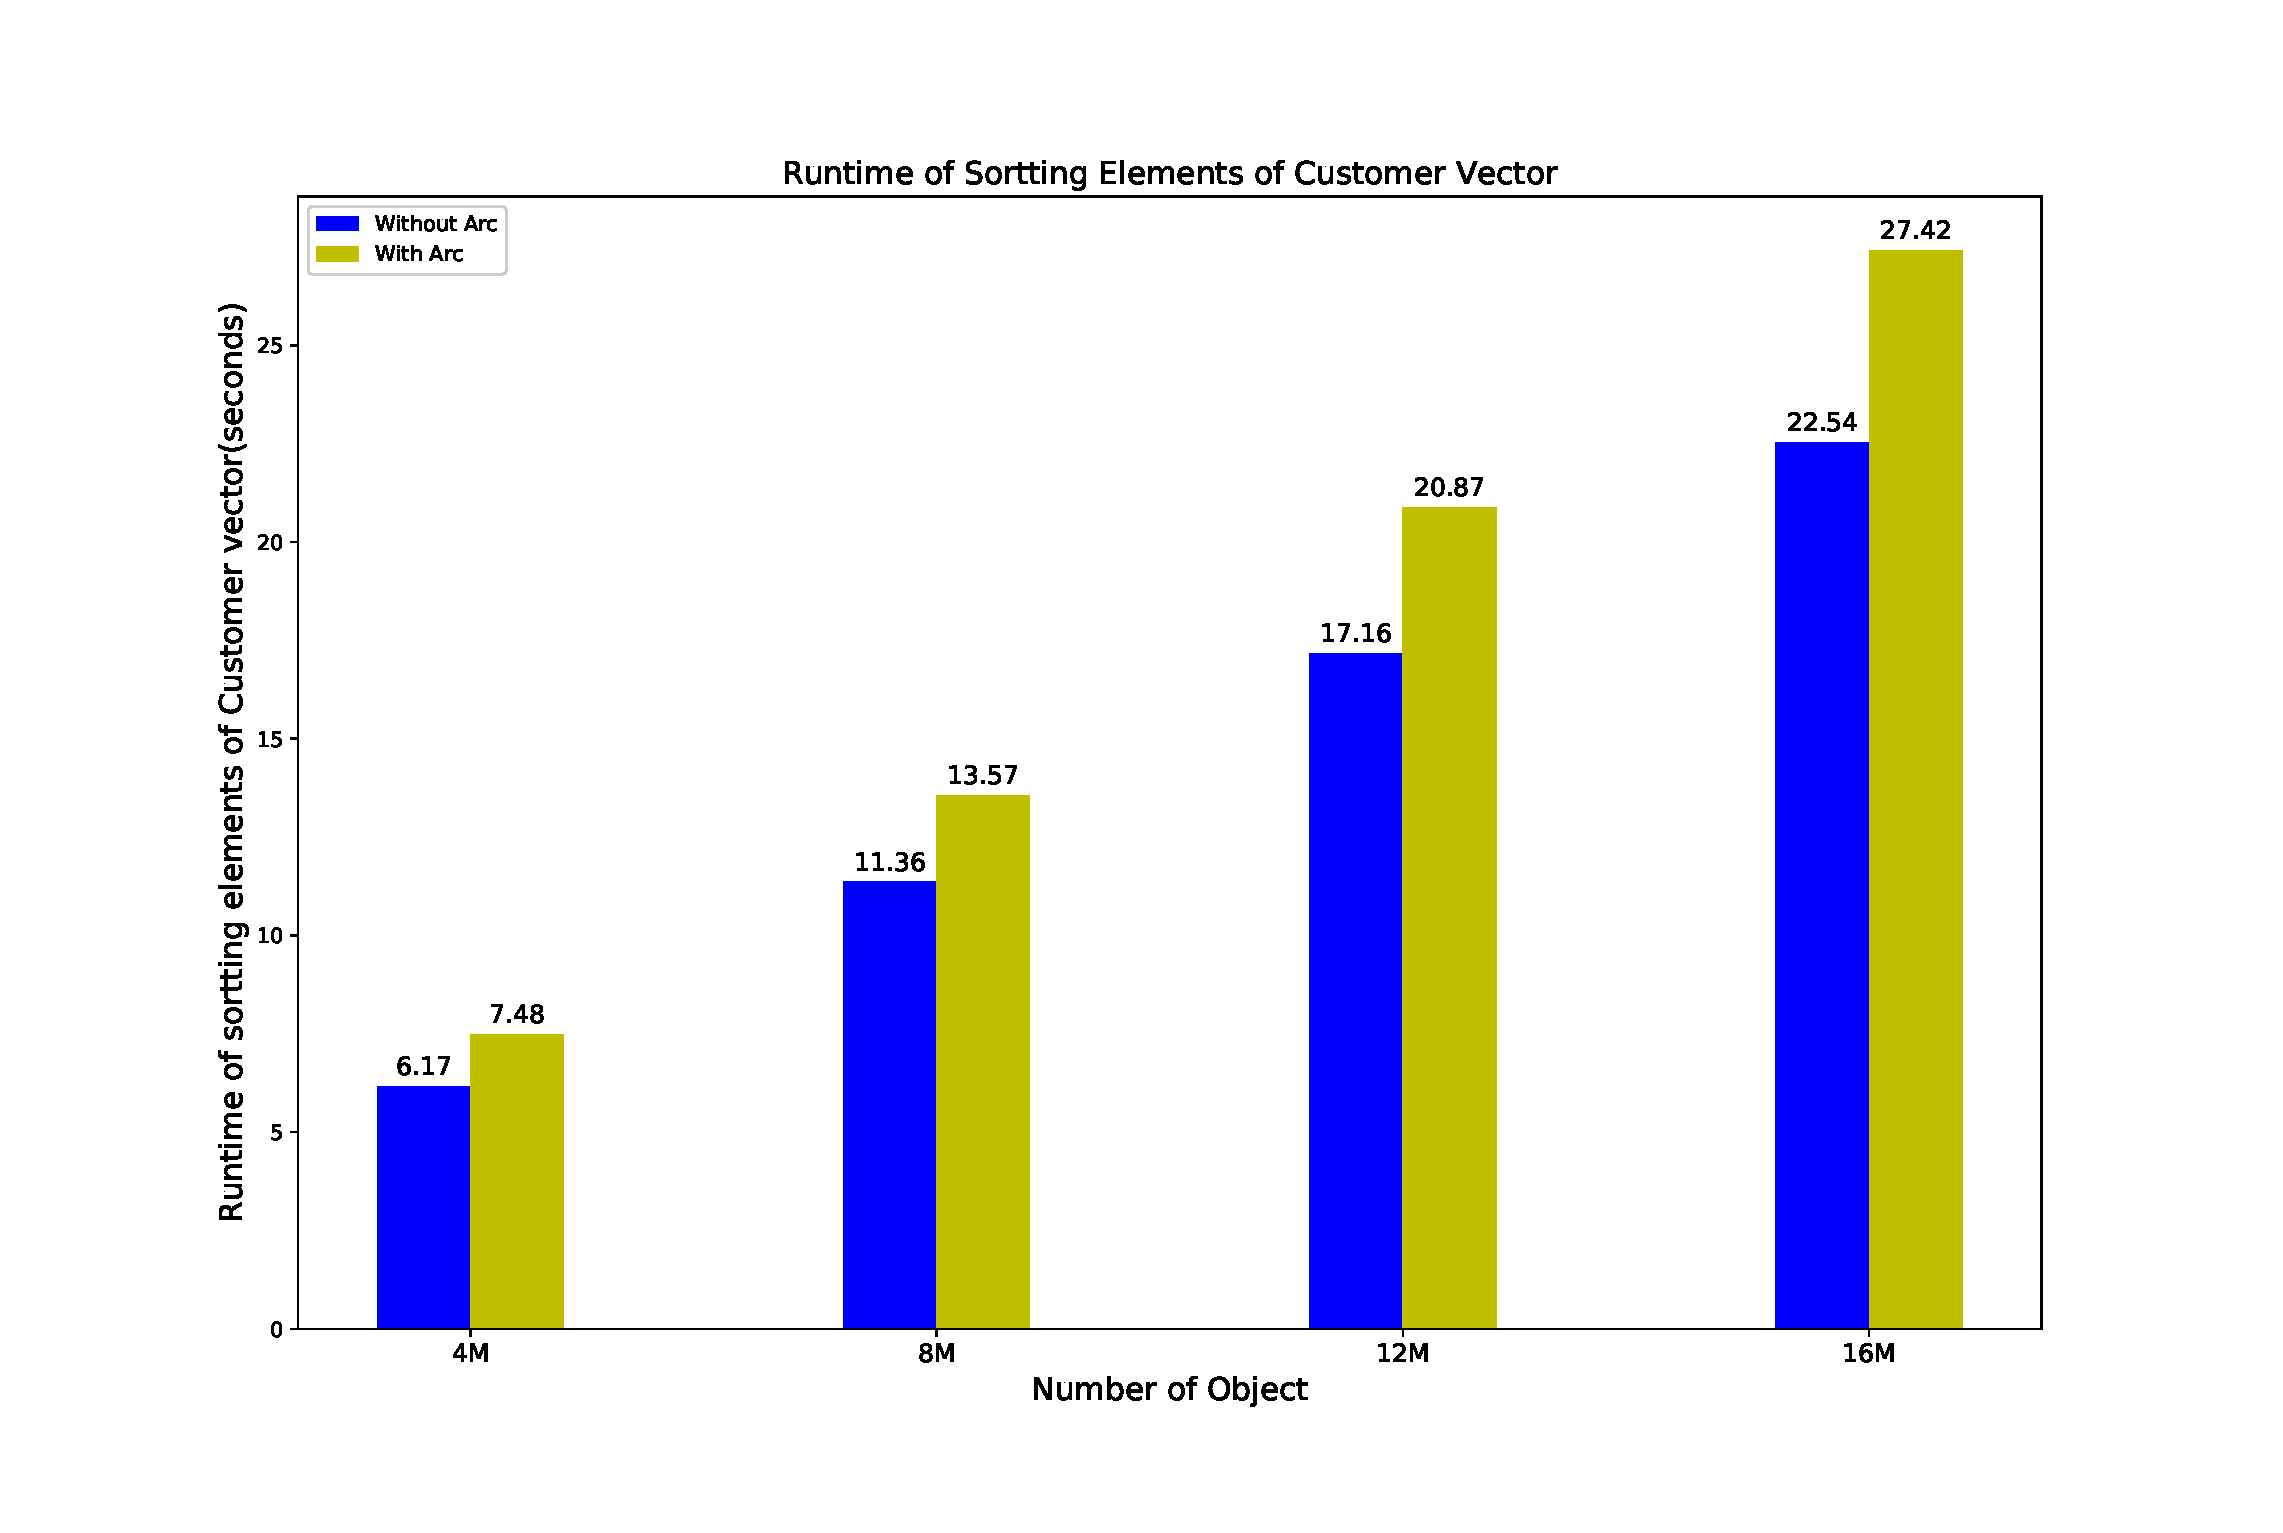
\includegraphics[width=1.1\textwidth]{images/rust_merge_sort.eps}
%                 \captionsetup{labelformat=empty}
%                 % \caption{\textbf{}}
%         \end{center}
%     \end{figure}
% \end{frame}

%%%%%%%%%%%%%%%%%%%%%%%%%%%%%%%%%%%%%%%%%%%%
%%%%%%%%%%%%%%%%%%%%%%%%%%%%%%%%%%%%%%%%%%%%

\begin{frame}[fragile]{Experiment 3: Merge-sort}
    \vspace{-0.55cm}
    \begin{figure}[hp]
        \centering
        \begin{center}
                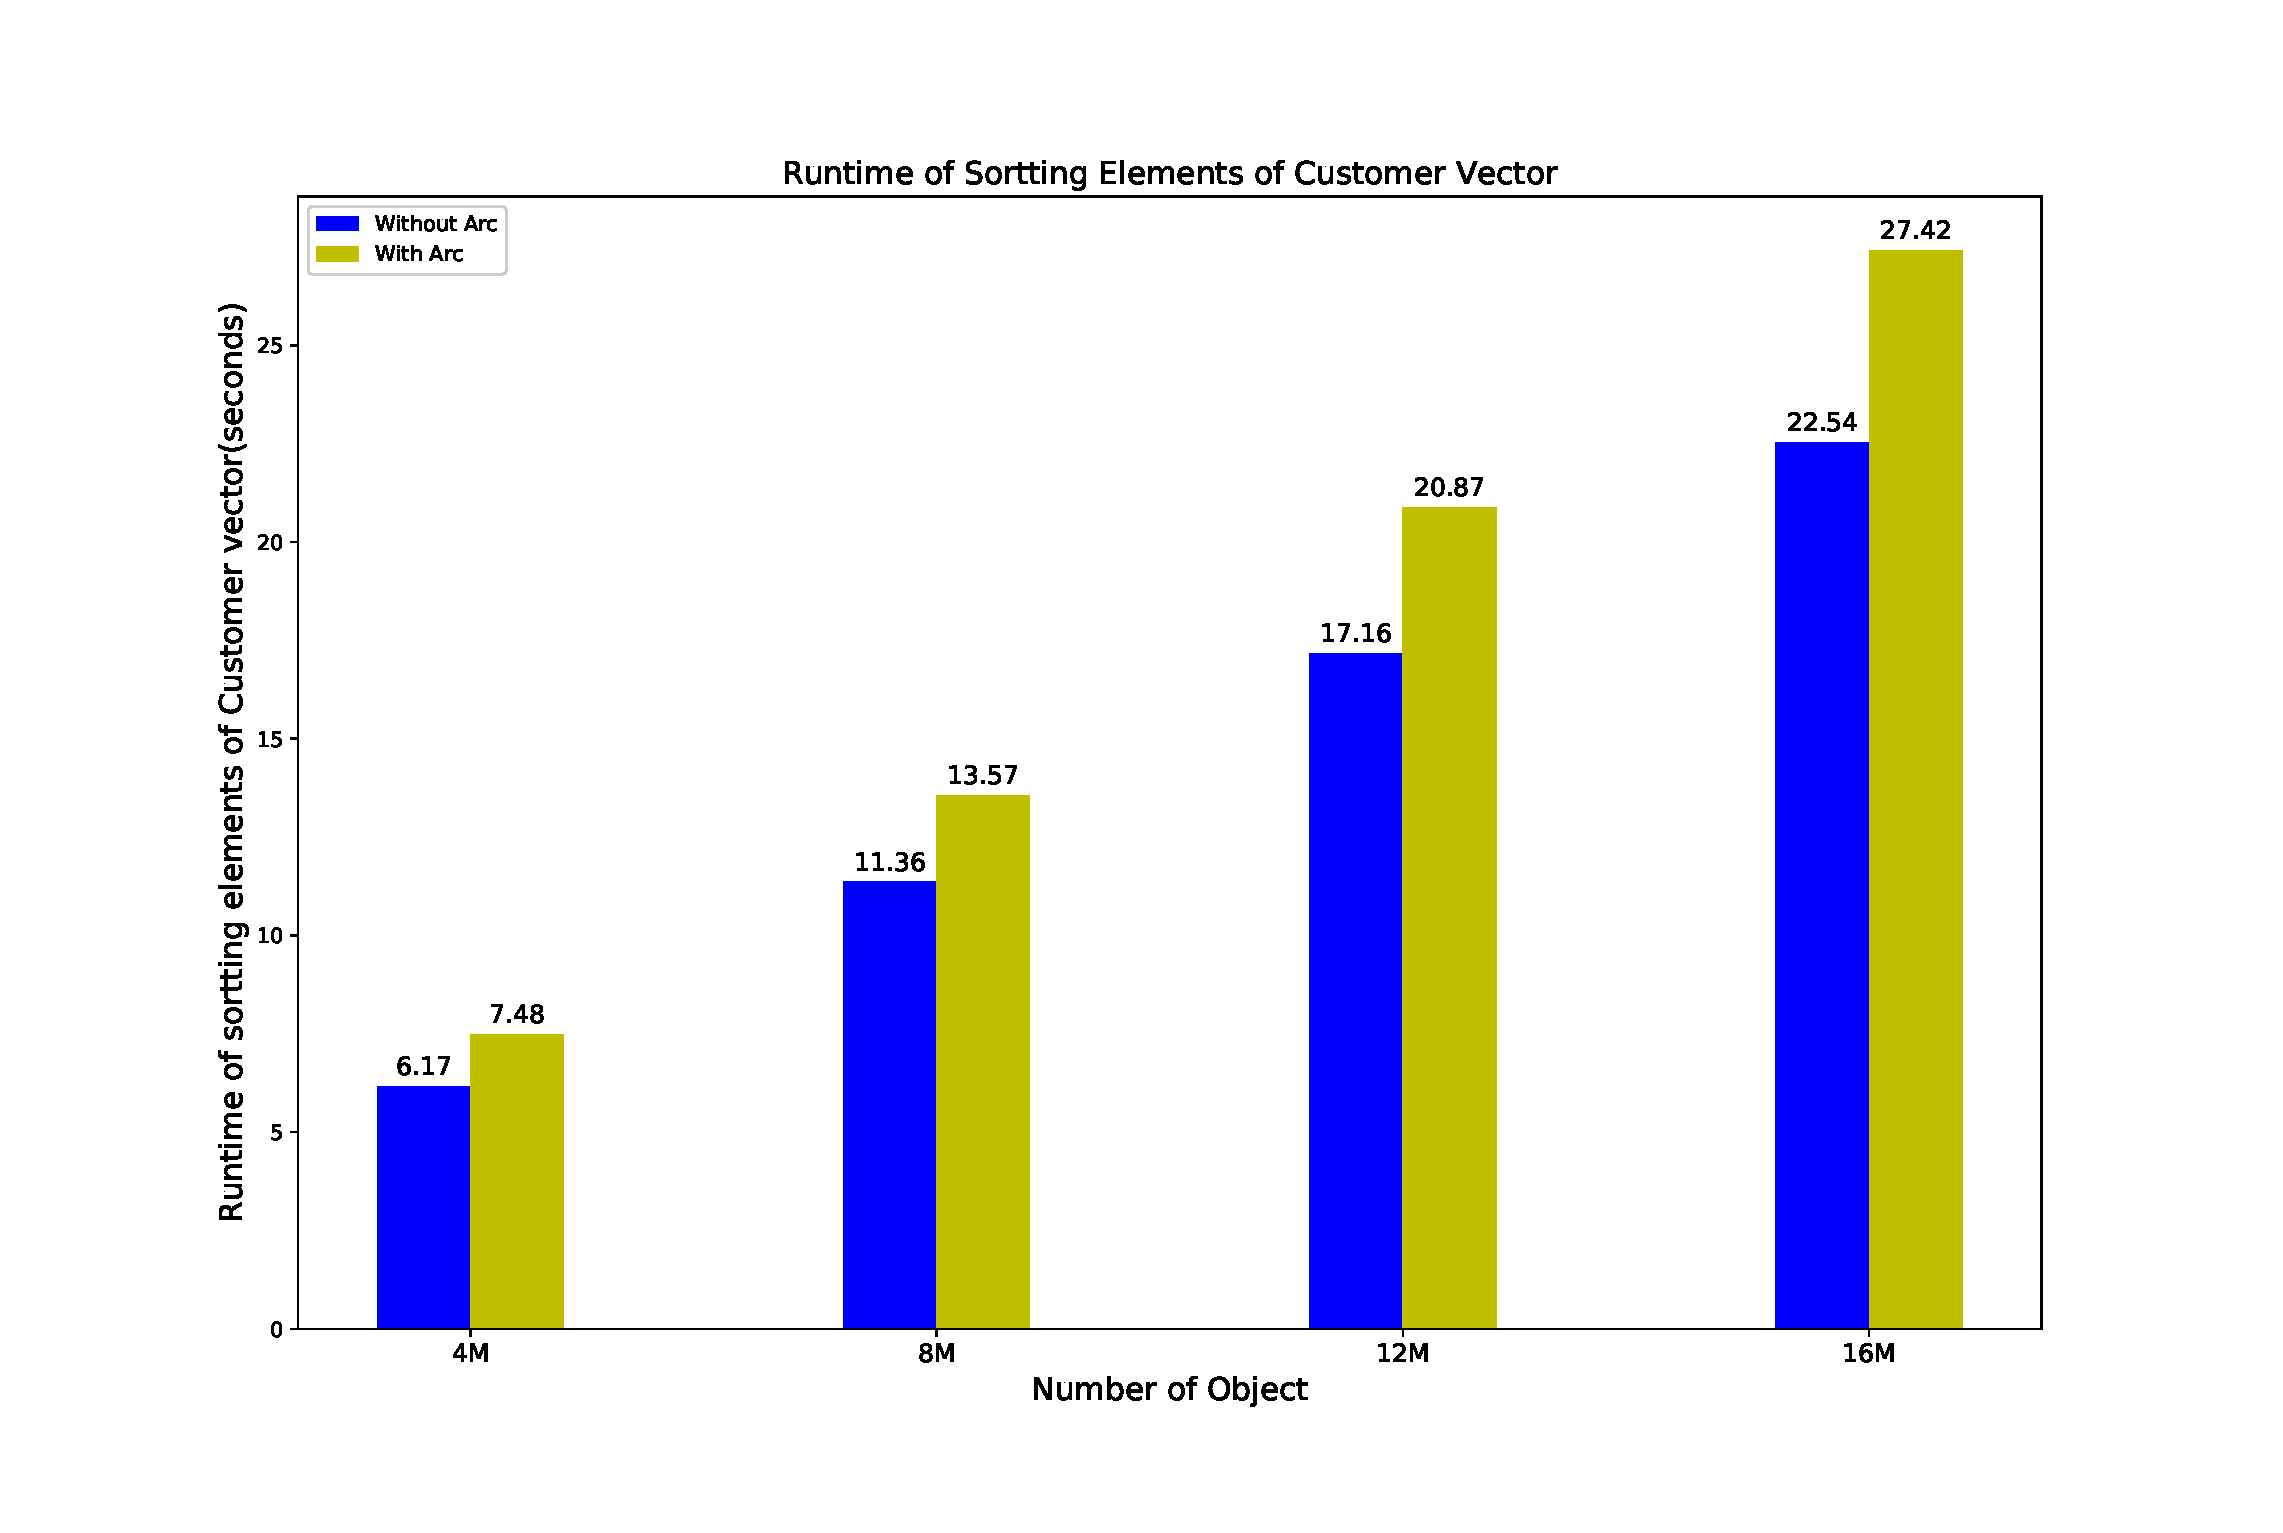
\includegraphics[width=0.8\textwidth]{images/rust_merge_sort.eps}
                \captionsetup{labelformat=empty}
                % \caption{\textbf{}}
        \end{center}
    \end{figure}
    \vspace{-0.95cm}
    \textbf{Result}
    \begin{itemize}
        \item Arc are about \blueb{21\%  slower} than normal reference.
    \end{itemize}
    \textbf{Discussion}
    \begin{itemize}
        \item Atomic Reference Counting needs to check reference count.
        \item Atomic operations are more expensive than ordinal operations.
    \end{itemize}

\end{frame}

%%%%%%%%%%%%%%%%%%%%%%%%%%%%%%%%%%%%%%%%%%%%
%%%%%%%%%%%%%%%%%%%%%%%%%%%%%%%%%%%%%%%%%%%%

\begin{frame}[fragile]{Experiment 4: Tree-aggregate}

    \textbf{Question}
    \begin{itemize}
        \item - What is performance hit of Tree-aggregate using Arc vs. deep-copy?
    \end{itemize}

    \vspace{0.5cm}

    \textbf{Evaluation}
    \begin{itemize}
        \item Share \blueb{elements} of complex object in multithreads
        \item \blueb{Atomic Reference Counting (Arc)} vs. \blueb{Deep copy}
        \item Measure \blueb{runtime of Tree-aggregate algorithm}
    \end{itemize}

\end{frame}

%%%%%%%%%%%%%%%%%%%%%%%%%%%%%%%%%%%%%%%%%%%%
%%%%%%%%%%%%%%%%%%%%%%%%%%%%%%%%%%%%%%%%%%%%

% \begin{frame}[t, fragile]{Experiment 4: Tree-aggregate}
%     \vspace{-0.7cm}
%     \begin{figure}[hp]
%         \centering
%         \begin{center}
%                 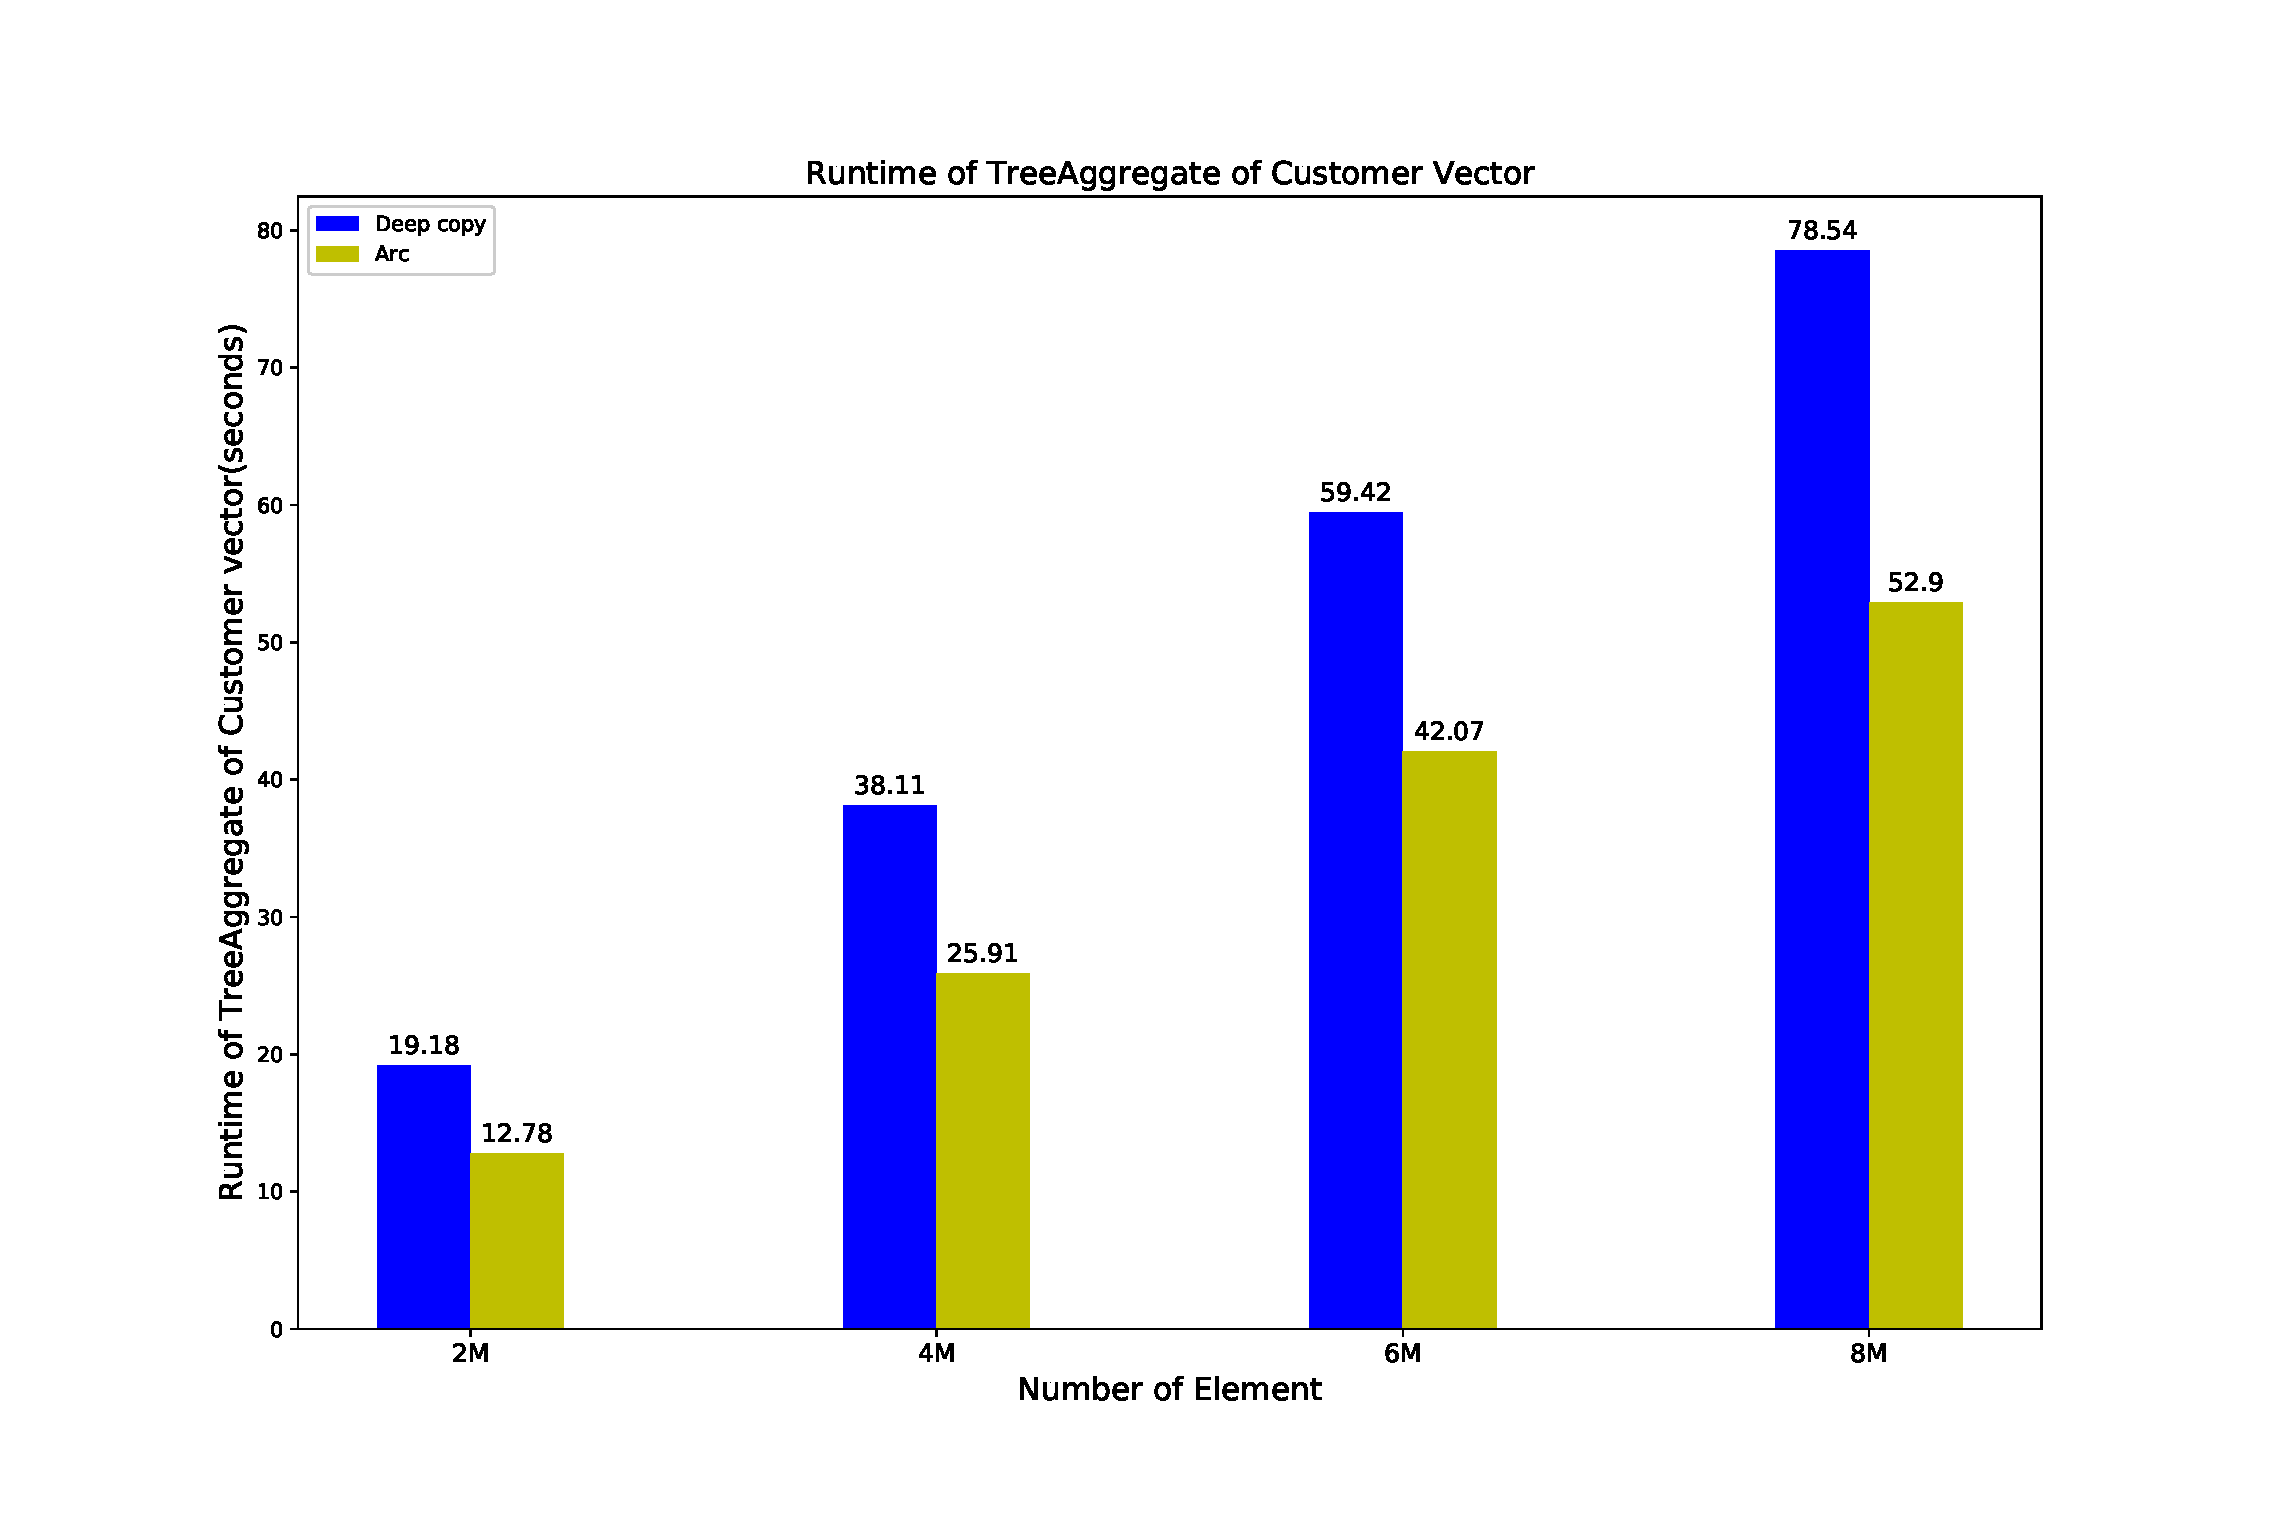
\includegraphics[width=1.1\textwidth]{images/rust_tree_aggregate.eps}
%                 \captionsetup{labelformat=empty}
%                 % \caption{\textbf{}}
%         \end{center}
%     \end{figure}
% \end{frame}

%%%%%%%%%%%%%%%%%%%%%%%%%%%%%%%%%%%%%%%%%%%%
%%%%%%%%%%%%%%%%%%%%%%%%%%%%%%%%%%%%%%%%%%%%

\begin{frame}[fragile]{Experiment 4: Tree-aggregate}
    \vspace{-0.5cm}
    \begin{figure}[hp]
        \centering
        \begin{center}
                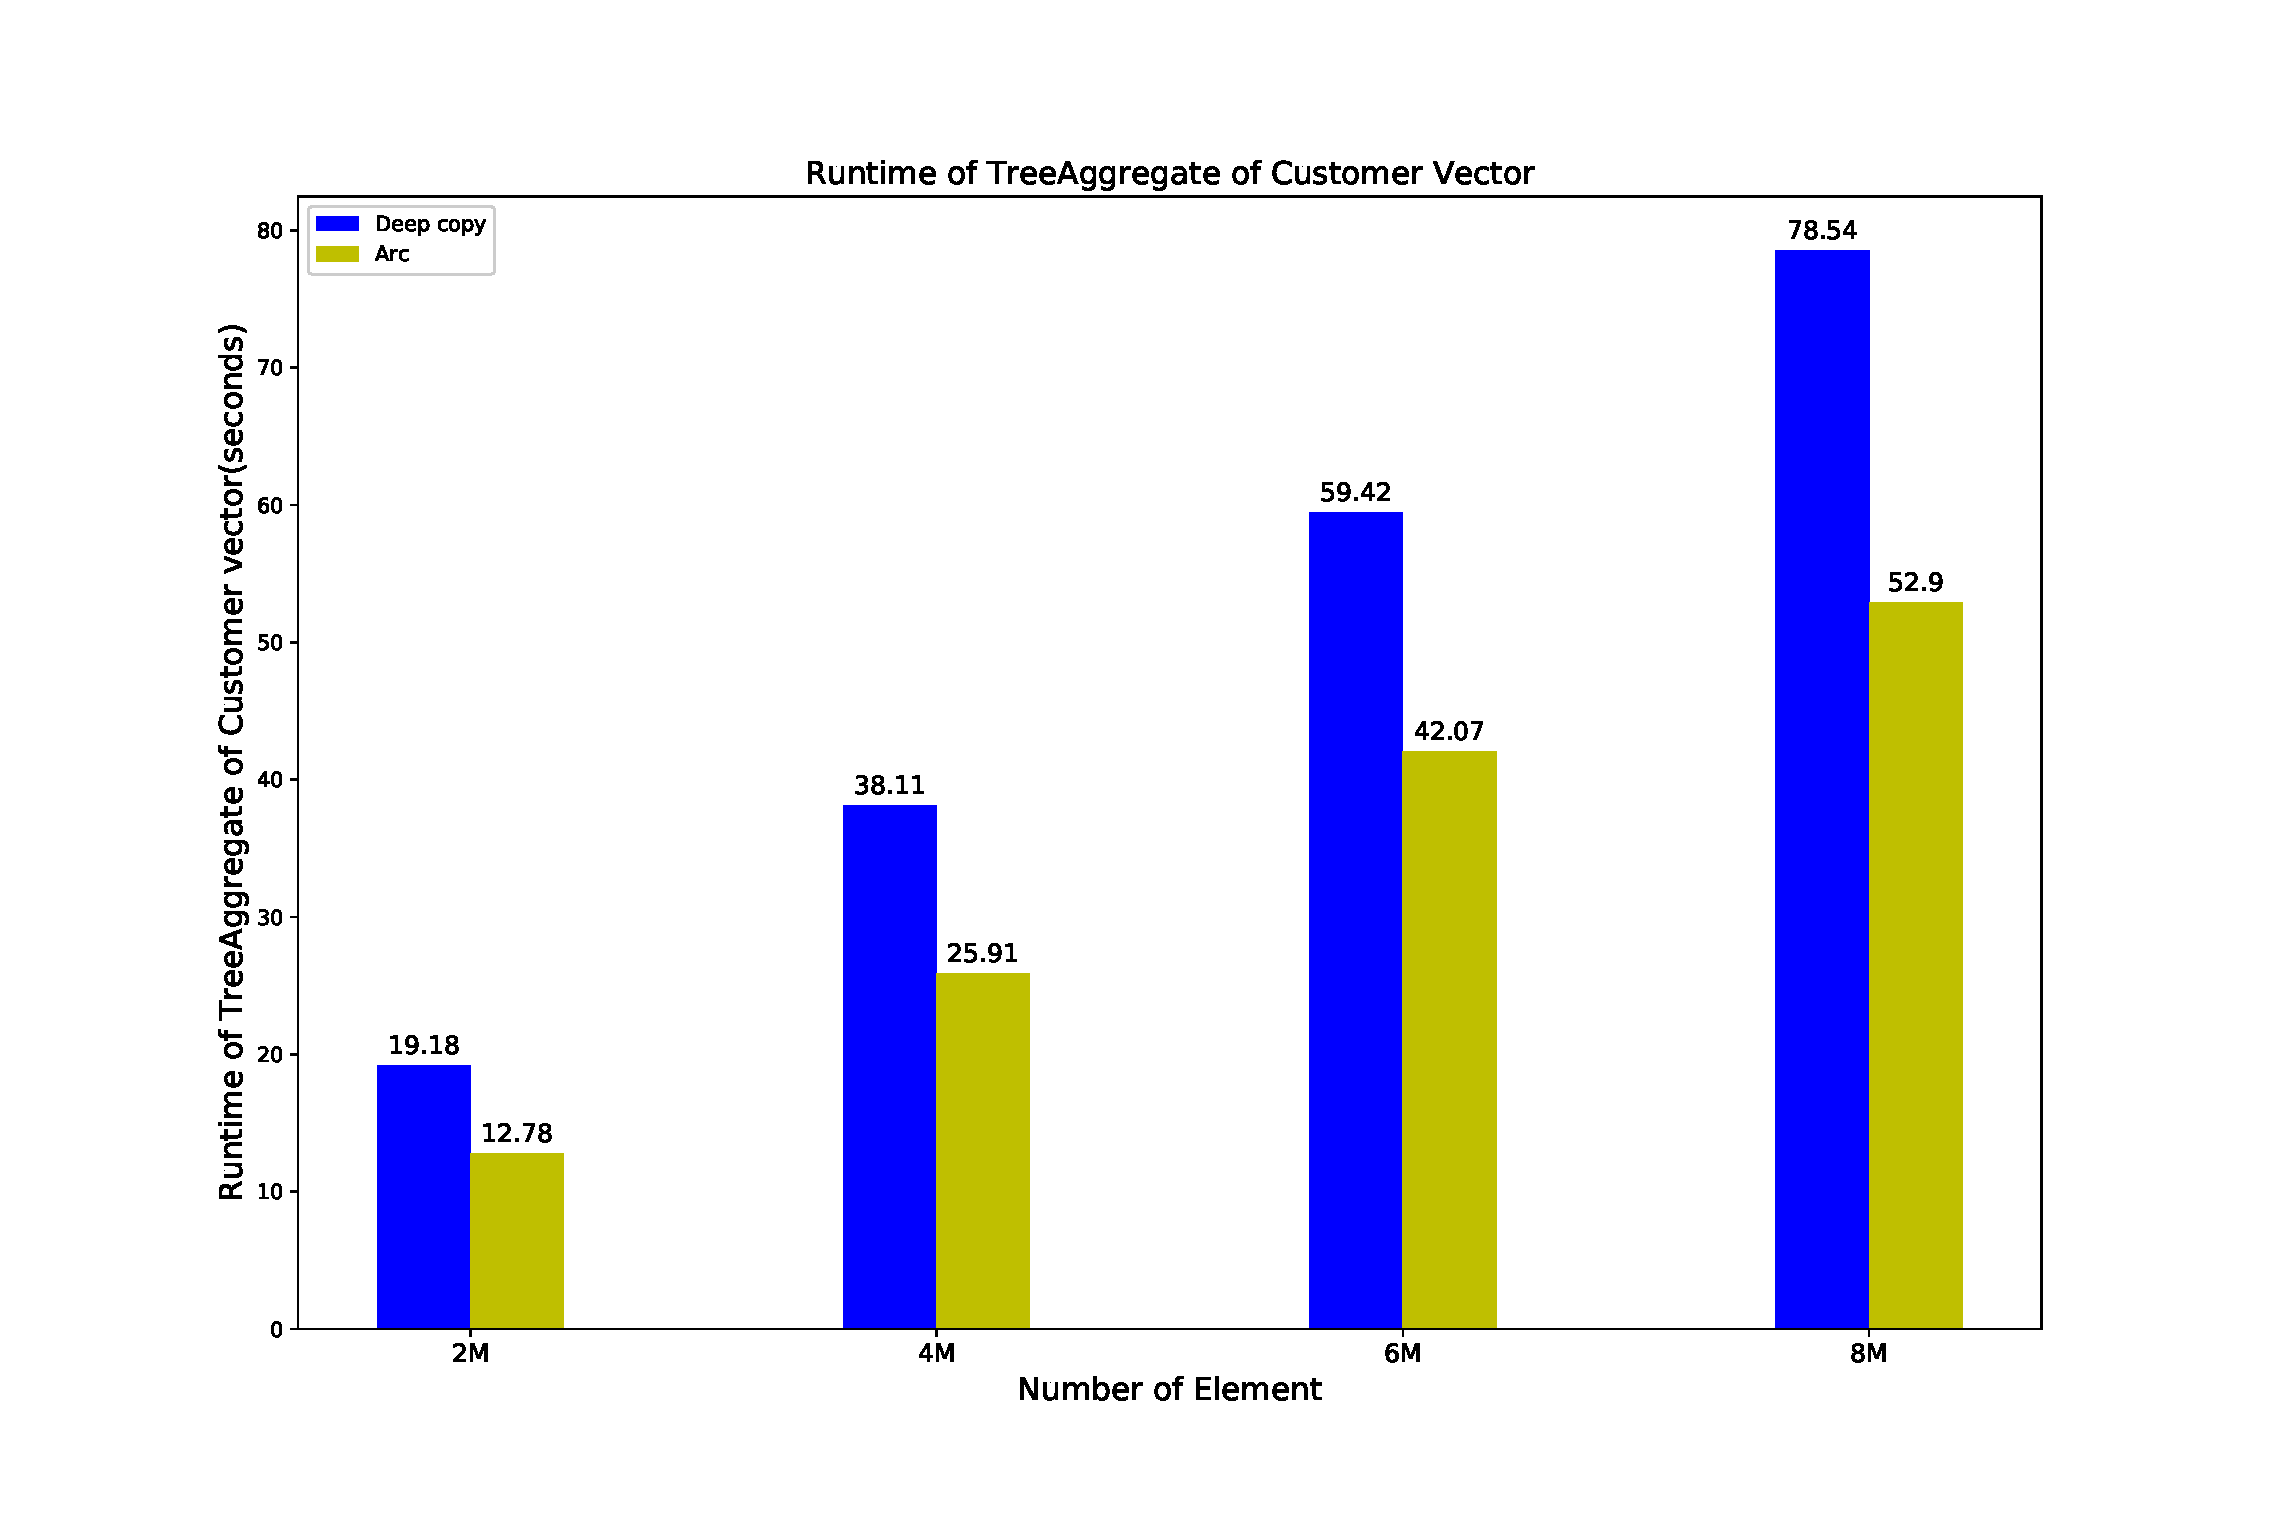
\includegraphics[width=0.85\textwidth]{images/rust_tree_aggregate.eps}
                \captionsetup{labelformat=empty}
                % \caption{\textbf{}}
        \end{center}
    \end{figure}
    \vspace{-1.1cm}
    \textbf{Result}
    \begin{itemize}
        \item Deep-copies are from \blueb{40\% to 50\% slower} than Arc.
    \end{itemize}

    \textbf{Discussion}
    \begin{itemize}
        \item Deep-copy of complex object is expensive.
        \item Performing deep-copy many times may lead to significant overhead.
    \end{itemize}

\end{frame}

%%%%%%%%%%%%%%%%%%%%%%%%%%%%%%%%%%%%%%%%%%%%
%%%%%%%%%%%%%%%%%%%%%%%%%%%%%%%%%%%%%%%%%%%%
\begin{frame}[fragile]{Experiment 5: K-Nearest-Neighbors (KNN)}

    \textbf{Question}
    \begin{itemize}
        \item - What is performance hit of Machine learning algorithms using Arc vs. deep-copy?
    \end{itemize}

    \vspace{0.5cm}

    \textbf{Evaluation}
    \begin{itemize}
        \item Document classification on Wikipedia page dataset
        \begin{itemize}
            \item Training set: \(100 \times 10^3 \) wiki pages
            \item Testing set: \(18 \times  10^3\) wiki pages
        \end{itemize}
        \item Preprocessing phase: calculating \blueb{Term-Frequencies (TFs)}
        \item String manipulation
        \item Measure runtime of \blueb{preprocessing time of KNN algorithms}
    \end{itemize}
\end{frame}

%%%%%%%%%%%%%%%%%%%%%%%%%%%%%%%%%%%%%%%%%%%%
%%%%%%%%%%%%%%%%%%%%%%%%%%%%%%%%%%%%%%%%%%%%

\begin{frame}[fragile]{Experiment 5: K-Nearest-Neighbors (KNN)}

    \blueb{Parameters}
    \begin{itemize}
        \item Data Acquisition
        \begin{itemize}
            \item \blueb{Atomic Reference Counting} (Arc)
            \item \blueb{Deep-copy}
        \end{itemize} 
        \vspace{0.5cm}
        % \item Strategy
        % \begin{itemize}
        %     \item keep intermediate objects in memory until owner is changed
        %     \item remove intermediate objects as soon as it is not needed
        % \end{itemize}
        % \vspace{0.5cm}
        \item Dimensions of feature matrices
        \begin{itemize}
            \item 15K
            \item 20K
            \item 25K
        \end{itemize} 
    \end{itemize}
\end{frame}

%%%%%%%%%%%%%%%%%%%%%%%%%%%%%%%%%%%%%%%%%%%%
%%%%%%%%%%%%%%%%%%%%%%%%%%%%%%%%%%%%%%%%%%%%

% \begin{frame}[fragile]{Experiment 5: K-Nearest-Neighbors}
%     \vspace{-0.7cm}
%     \begin{figure}[hp]
%         \centering
%         \begin{center}
%                 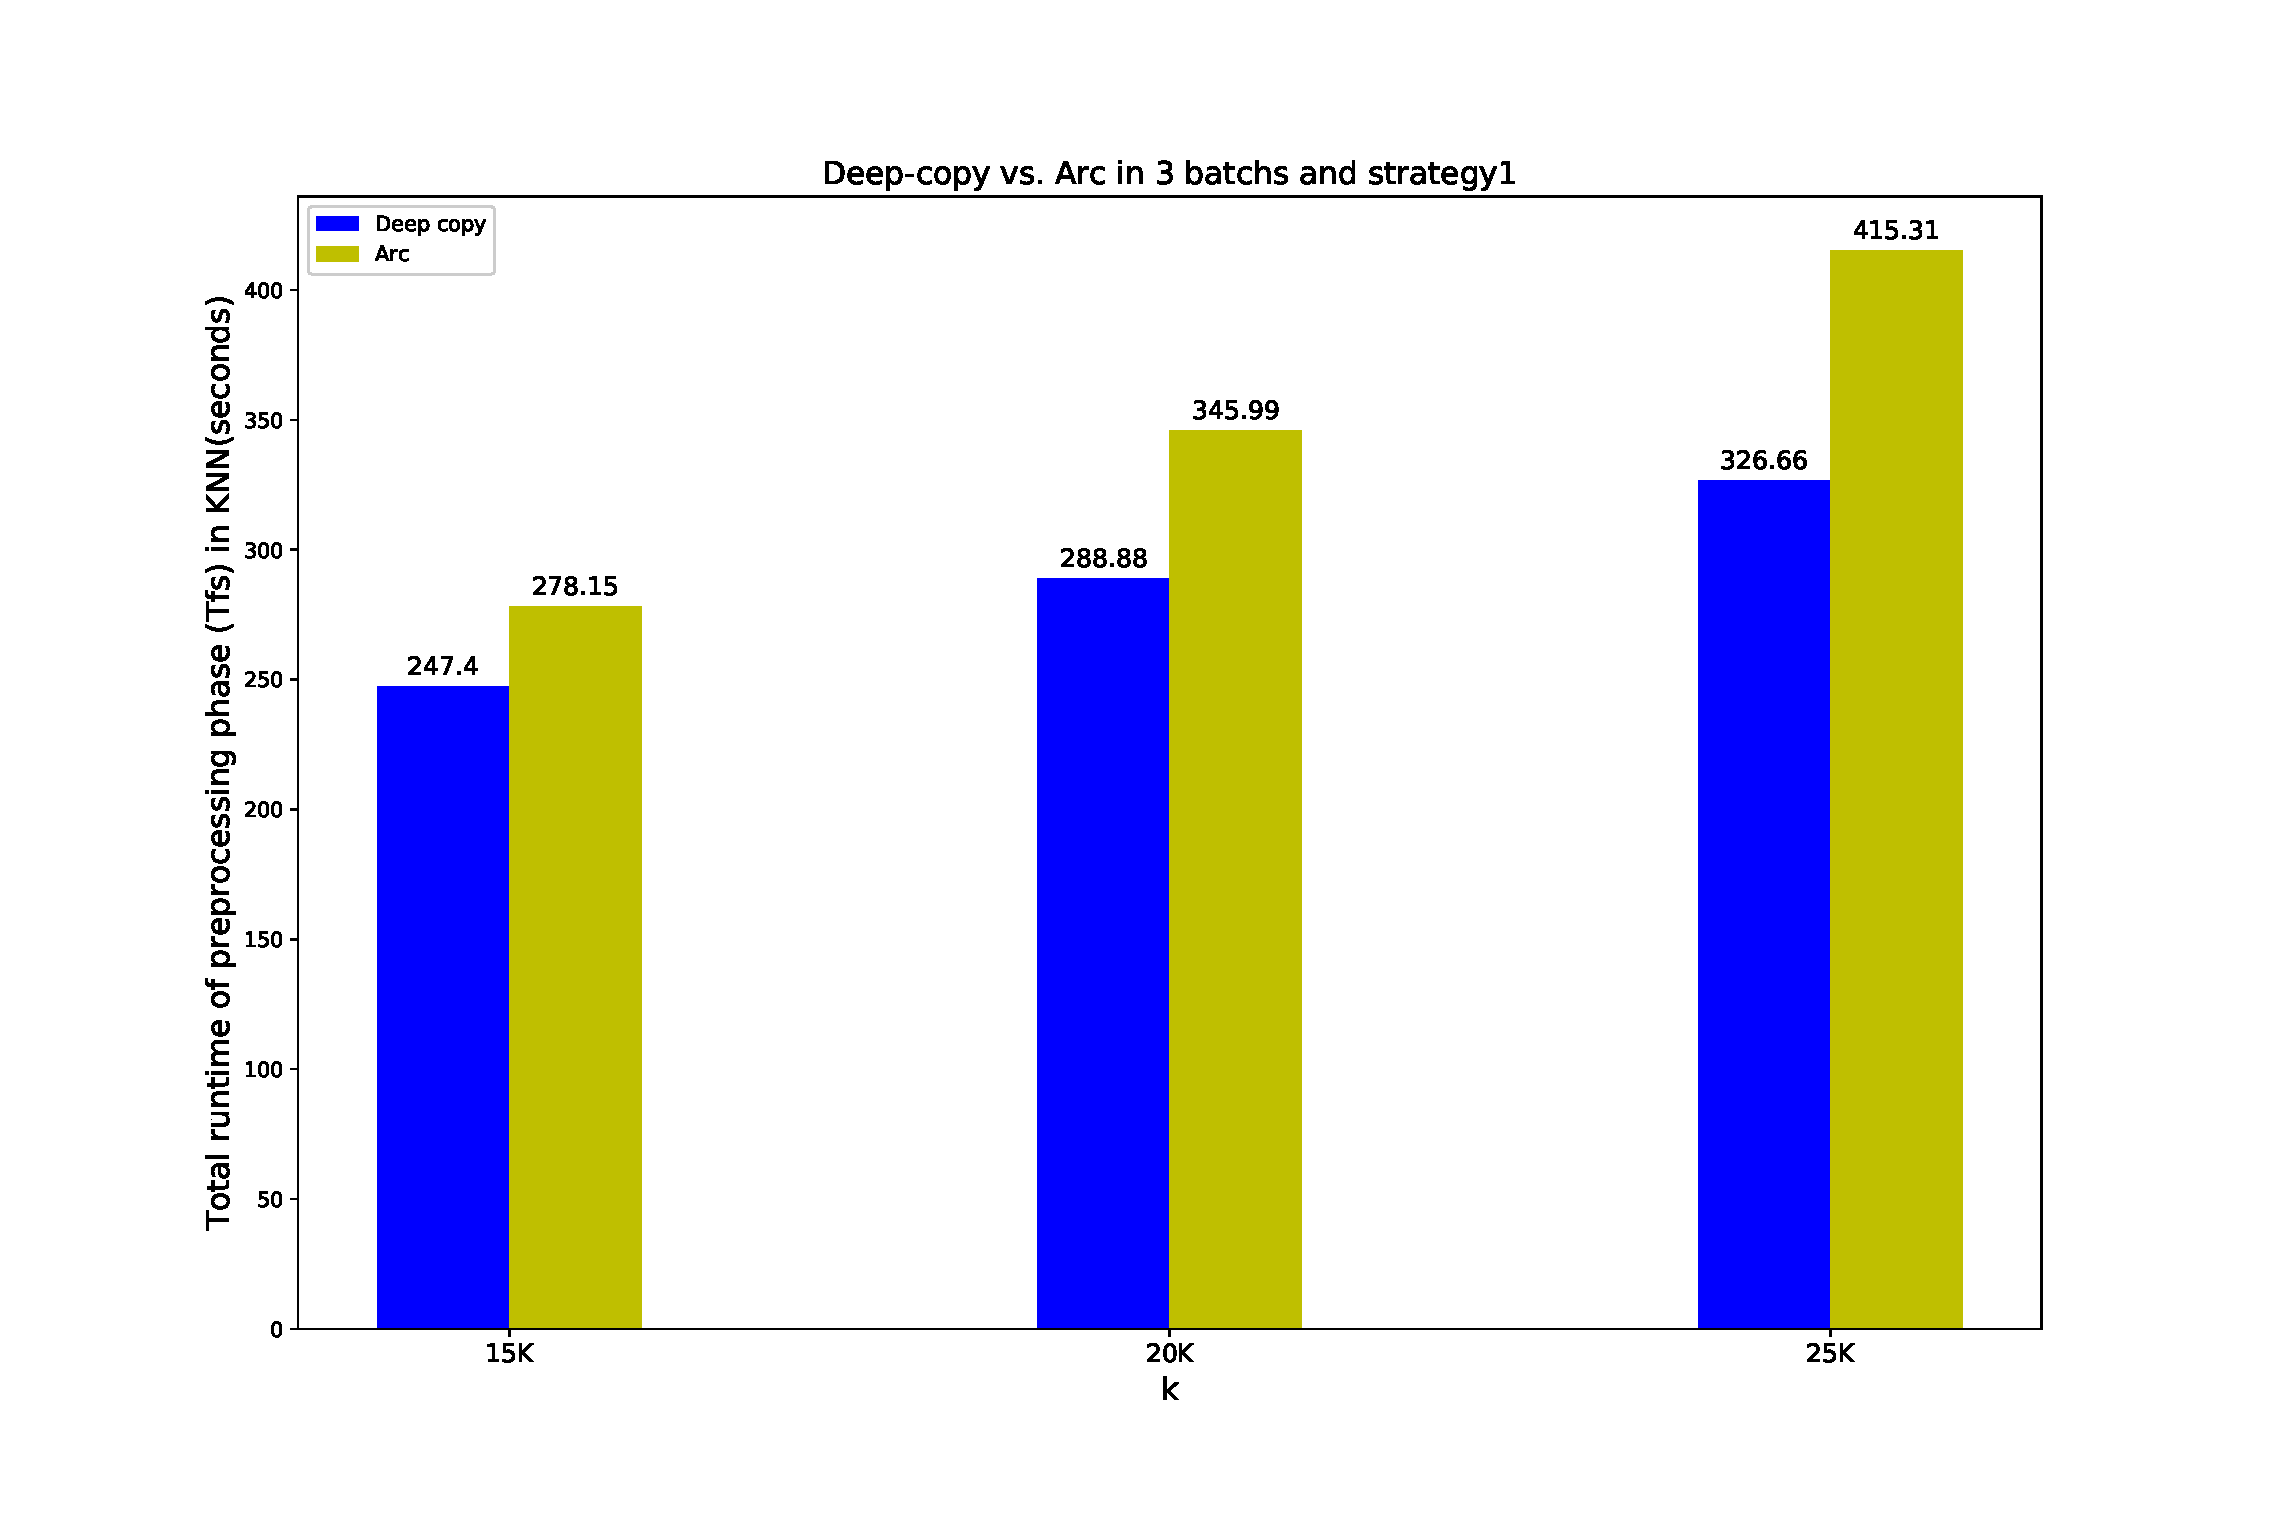
\includegraphics[width=1.1\textwidth]{images/deepcopy_vs_arc.eps}
%                 \captionsetup{labelformat=empty}
%                 % \caption{\textbf{}}
%         \end{center}
%     \end{figure}
%     
% \end{frame}

%%%%%%%%%%%%%%%%%%%%%%%%%%%%%%%%%%%%%%%%%%%%
%%%%%%%%%%%%%%%%%%%%%%%%%%%%%%%%%%%%%%%%%%%%

% \begin{frame}[fragile]{Experiment 5: K-Nearest-Neighbors}
%     \vspace{-0.7cm}
%     \begin{figure}[hp]
%         \centering
%         \begin{center}
%                 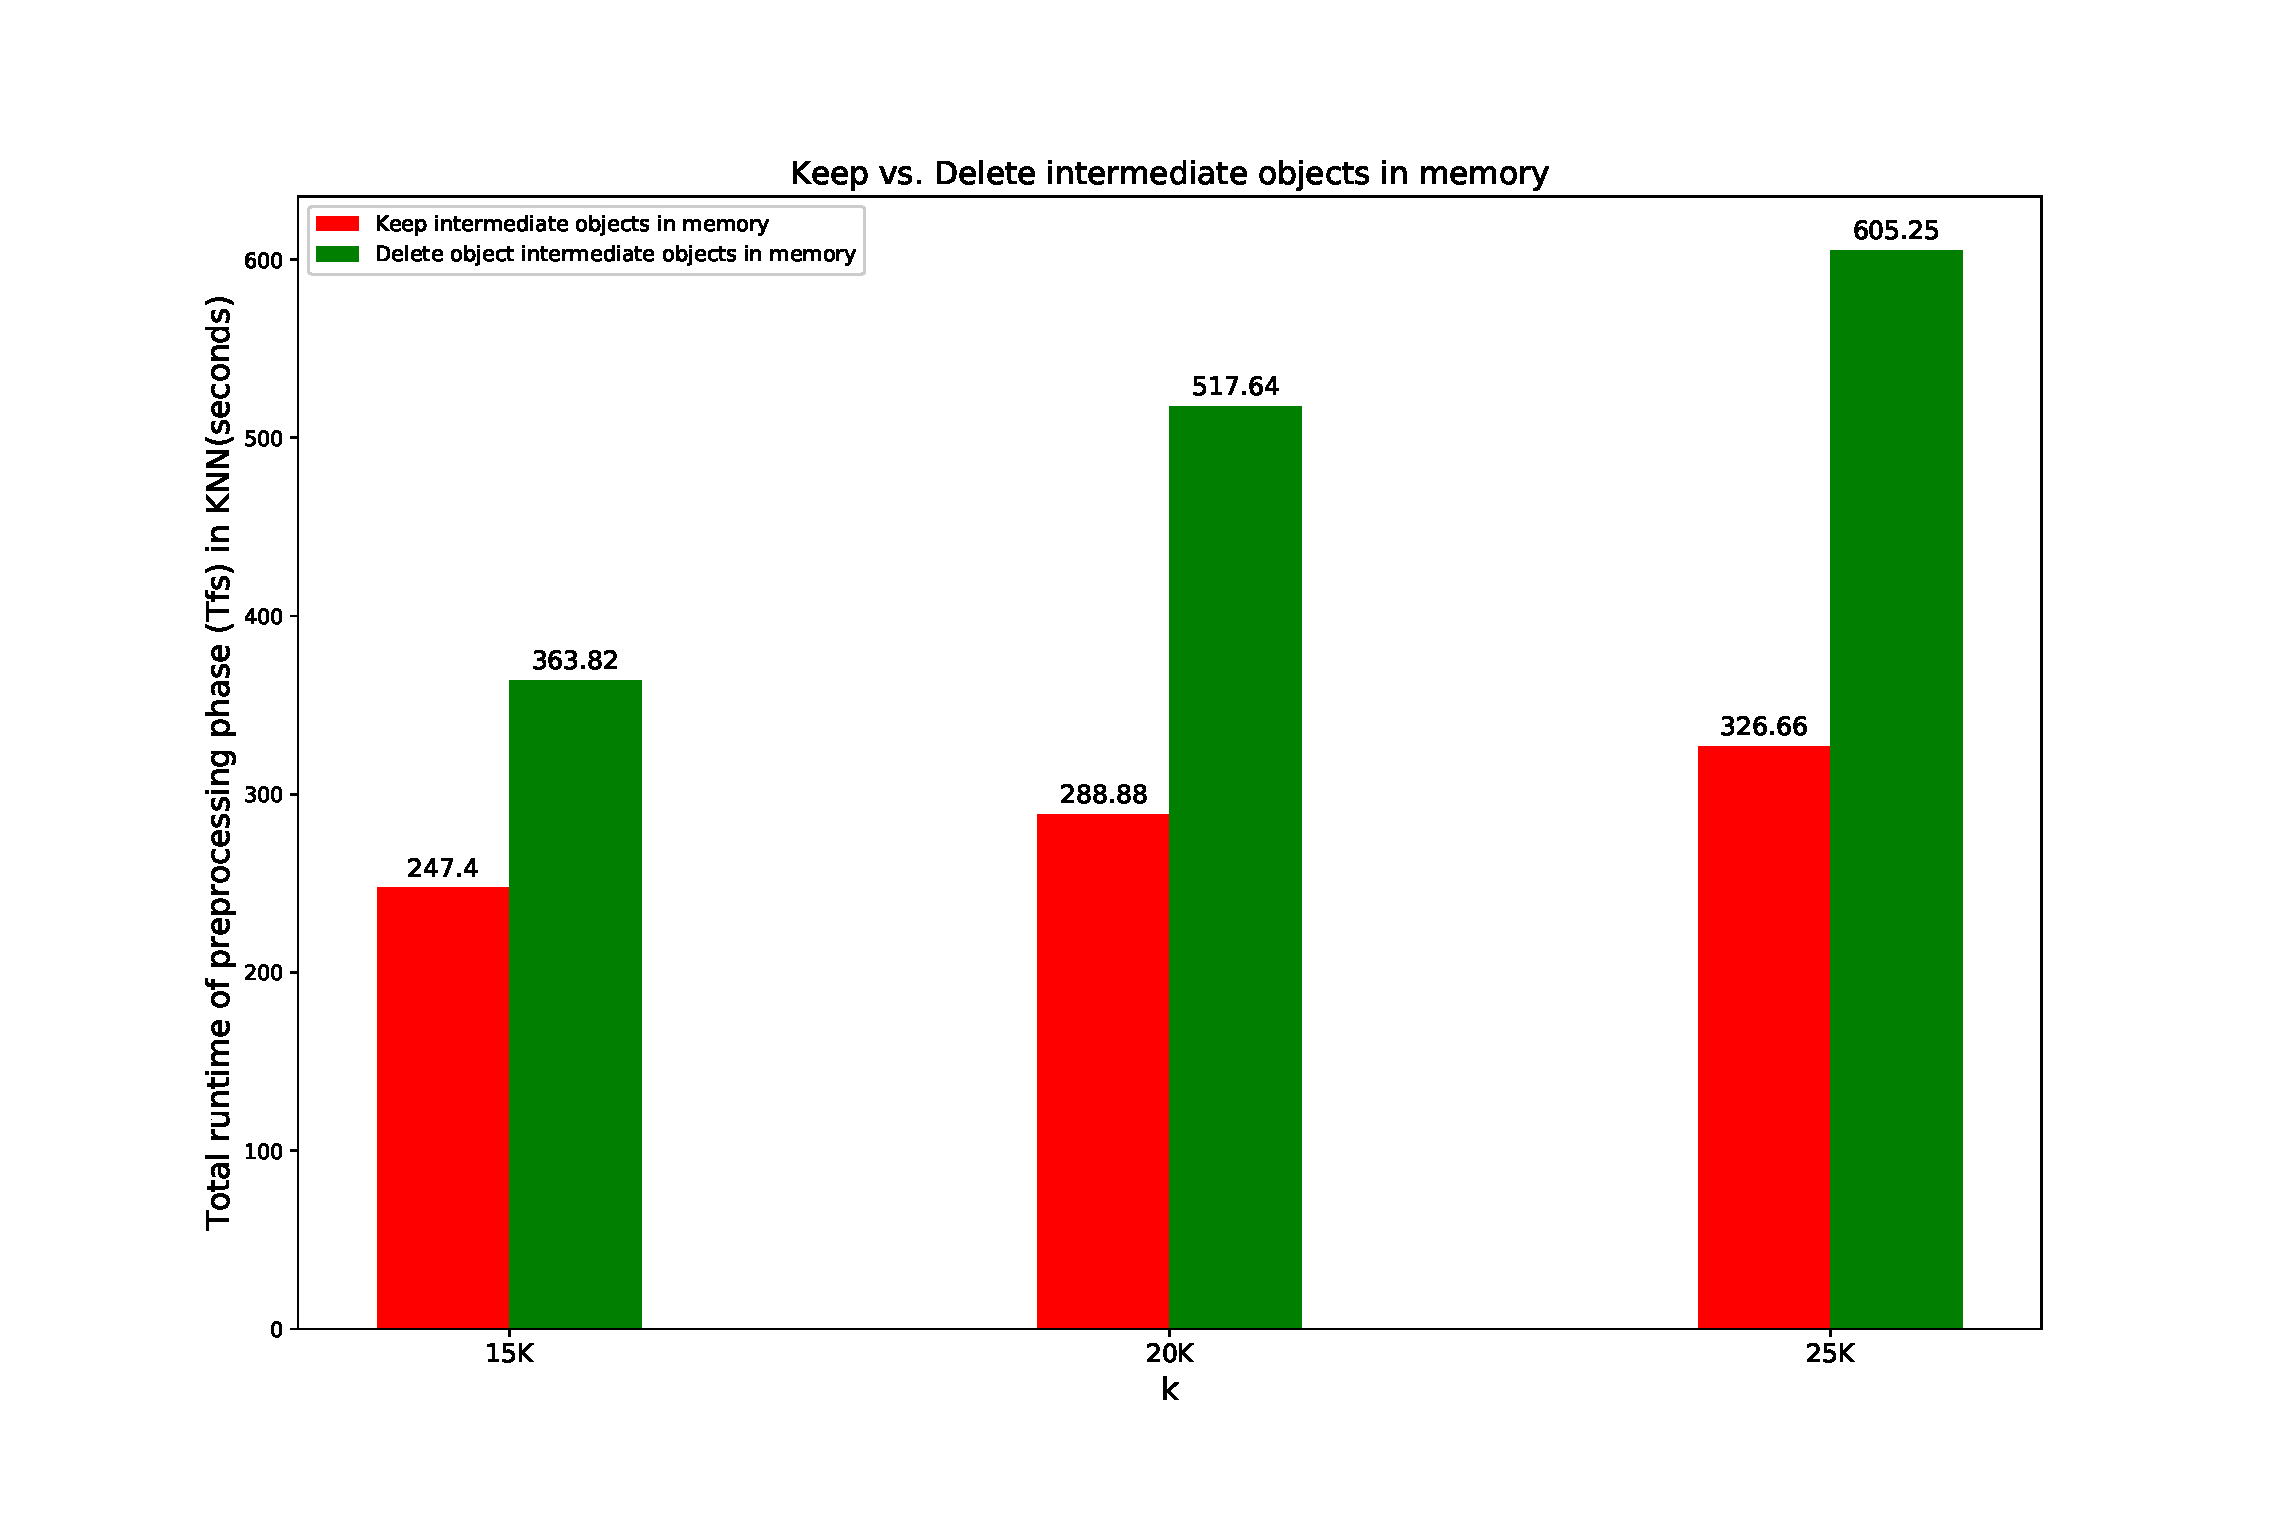
\includegraphics[width=1.1\textwidth]{images/strategy1_vs_strategy2.eps}
%                 \captionsetup{labelformat=empty}
%                 % \caption{\textbf{}}
%         \end{center}
%     \end{figure}
    
% \end{frame}

%%%%%%%%%%%%%%%%%%%%%%%%%%%%%%%%%%%%%%%%%%%%
%%%%%%%%%%%%%%%%%%%%%%%%%%%%%%%%%%%%%%%%%%%%


\begin{frame}[fragile]{Experiment 5: K-Nearest-Neighbors - Preprocessing Time}
    \vspace{-0.4cm}
    \begin{figure}[hp]
        \centering
        \begin{center}
                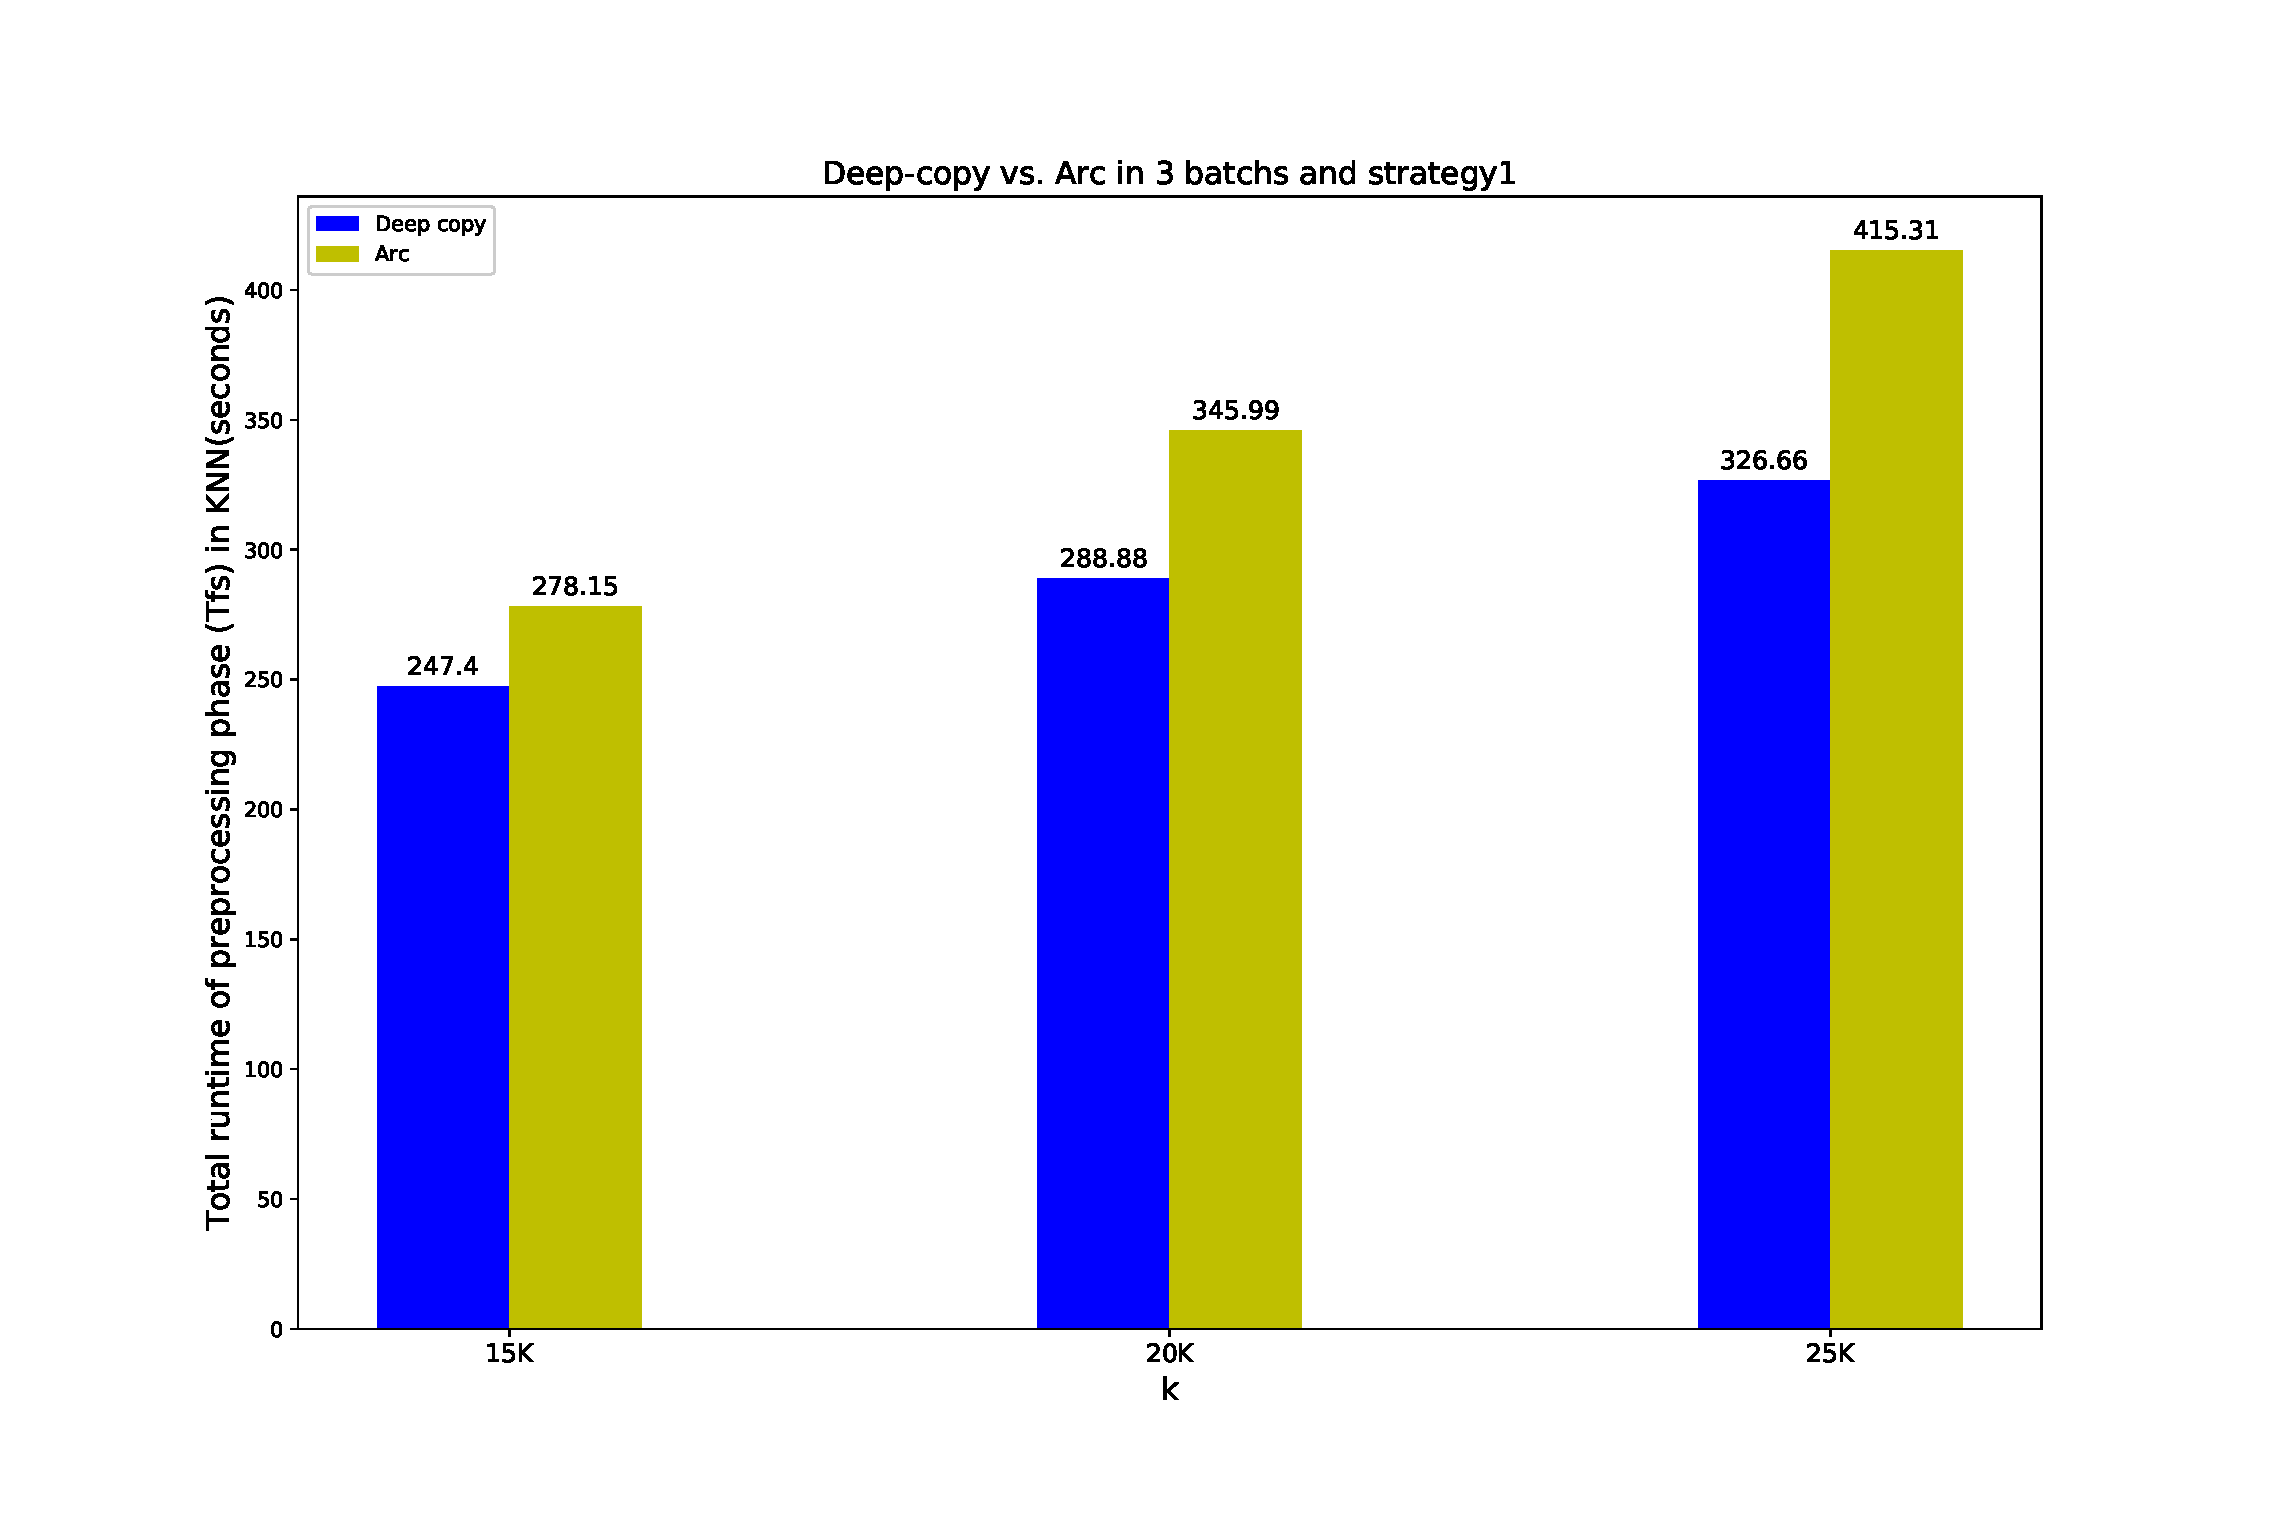
\includegraphics[width=0.8\textwidth]{images/deepcopy_vs_arc.eps}
                \captionsetup{labelformat=empty}
                % \caption{\textbf{}}
        \end{center}
    \end{figure} 
    \vspace{-0.9cm}
    \textbf{Result}
    \begin{itemize}
        \item \blueb{Arc} is \blueb{at most 27\% slower} than deep-copy.
        % \item Removing intermediate objects is \blueb{at most 85\% slower} than keeping the objects.
    \end{itemize}

    \textbf{Discussion}
    \begin{itemize}
        \item Deep-copying String is cheaper operation than Arc: 
        \begin{itemize}
            \item Relatively simple object
            \item Contiguously allocated
        \end{itemize}
        \item Overhead using Arc may become more significant as size of data increases
        % \item More frequent deallocation of intermediate objects may lead to overhead.
    \end{itemize} 
\end{frame}


%%%%%%%%%%%%%%%%%%%%%%%%%%%%%%%%%%%%%%%%%%%%
%%%%%%%%%%%%%%%%%%%%%%%%%%%%%%%%%%%%%%%%%%%%

\begin{frame}[fragile]{Findings}

\textbf{Arc vs. Deep-Copy}

    \begin{itemize}
        \item Use Arc instead of deep-copy when \blueb{complexity of objects is large}.
        \item Use deep-copy when dealing with \blueb{low complex objects/primitive types} like String.
    \end{itemize}

\textbf{Arc vs. Normal Reference}

    \begin{itemize}

        \item Use normal reference rather than Reference Counting whenever it is possible.
        \item \blueb{Avoid using Arc} when we can use reference.
    \end{itemize}
\end{frame}

%%%%%%%%%%%%%%%%%%%%%%%%%%%%%%%%%%%%%%%%%%%%
%%%%%%%%%%%%%%%%%%%%%%%%%%%%%%%%%%%%%%%%%%%%

\begin{frame}[fragile]{Conclusion}
    \begin{itemize}
        \item We have seen that impact of memory memory Management is very large, 
              especially when working on High Complex Object structures and large volume of data set. 

        \item Using a System Language like Rust is very promising to avoid using large CPU computation for memory management. 
        \item When using Rust writing memory-safe multithreaded code is fairly easy.
         
    \end{itemize}
\end{frame}
\end{document}
